\chapter{Messergebnisse}
\label{ergebnisse}

Im Rahmen dieses Kapitels wird auf die Messergebnisse eingegangen, die im Zuge der Performance-Analyse der Datenbanksysteme erzielten werden. Dabei werden zuerst die Latenz- und Durchsatzwerte der Messungen für die Datenbanksysteme im Rahmen der  Messreihen aufgeführt und besprochen. 

Für die erzielten Latenzwerten werden neben der durchschnittlichen Latenz (Mean) einer gebenchmarkten Operation auch das 25. (p25), 50. (p50), 75. (p75), 95. (p95) und 99. (p99) Perzentil aufgeführt sowie die höchste gemessene Latenz (Max.). Für den Vergleich der Ergebnisse der Datenbanksysteme wird allerdings hauptsächlich die Durchschnittslatenz (Mean) herangezogen. 

Beim Durchsatz wird hingegen lediglich dessen Durchschnitt aufgeführt. Die Darstellung und Besprechung der Ergebnisse der Messreihen erfolgt dabei in derselben Reihenfolge, wie sie bereits in \autoref{analyse:messreihen} aufgeführt werden. 

Die in diesem Kapitel erzielten Ergebnisse bilden dabei die Basis der detaillierten Auswertung und Einordnung der Performance der Datenbanksysteme im nächsten Kapitel (\autoref{auswertung}).

\section{Linkbench-10M-Const}
\label{ergebnisse:10m_const}
Dieser Abschnitt führt Latenz- und Durchsatzwerte auf, die im Rahmen dieser Messreihe für die Operationen der jeweiligen Datenbanksysteme Db2 Graph Beta 3, Db2 Graph V11.5.6.0 und Neo4j erzielt werden. Dabei wird auf Basis eines kleinen konstant verteilten Datensatzes gearbeitet.

\subsection{Latenz}

Die \autoref{tab:latenz_10m_const:beta3} stellt hier die für Db2 Graph Beta 3 gemessen Ergebnisse dar, während in \autoref{tab:latenz_10m_const:ga} die für Db2 Graph V11.5.6.0 ermittelten Latenz aufgeführt werden. Neo4j Latenzwerte für diese Messreihe werden in \autoref{tab:latenz_10m_const:neo4j} abgebildet.

\begin{table}[!ht]
\centering
\resizebox{\textwidth}{!}{
\begin{tabular}{l|r|r|r|r|r|r|r}
\hline
\rowcolor[HTML]{EFEFEF} 
\multicolumn{1}{c|}{\cellcolor[HTML]{EFEFEF}\textbf{Operation}} &
\multicolumn{1}{c|}{\cellcolor[HTML]{EFEFEF}\textbf{Mean}} &
\multicolumn{1}{c|}{\cellcolor[HTML]{EFEFEF}\textbf{p25}} &
\multicolumn{1}{c|}{\cellcolor[HTML]{EFEFEF}\textbf{p50}} &
\multicolumn{1}{c|}{\cellcolor[HTML]{EFEFEF}\textbf{p75}} &
\multicolumn{1}{c|}{\cellcolor[HTML]{EFEFEF}\textbf{p95}} &
\multicolumn{1}{c|}{\cellcolor[HTML]{EFEFEF}\textbf{p99}} &
\multicolumn{1}{c}{\cellcolor[HTML]{EFEFEF}\textbf{Max.}} \\ \hline
getNode & 6,16ms & {[}4,5{]}ms & {[}5,6{]}ms & {[}7,8{]}ms & {[}10,11{]}ms & {[}15,16{]}ms & 10.213,70ms \\
getLink & 7,79ms & {[}5,6{]}ms & {[}7,8{]}ms & {[}9,10{]}ms & {[}12,13{]}ms & {[}19,20{]}ms & 917,72ms \\
countLink & 10,72ms & {[}8,9{]}ms & {[}10,11{]}ms & {[}12,13{]}ms & {[}16,17{]}ms & {[}23,24{]}ms & 448,41ms \\
getLinkList & 10,83ms & {[}8,9{]}ms & {[}10,11{]}ms & {[}12,13{]}ms & {[}17,18{]}ms & {[}23,24{]}ms & 409,11ms \\ \hline
\end{tabular}
}
\caption{Latenz Linkbench-10M-Const Db2 Graph Beta 3}
\label{tab:latenz_10m_const:beta3}
\end{table}

\begin{table}[!ht]
\centering
\resizebox{\textwidth}{!}{
\begin{tabular}{l|r|r|r|r|r|r|r}
\hline
\rowcolor[HTML]{EFEFEF} 
\multicolumn{1}{c|}{\cellcolor[HTML]{EFEFEF}\textbf{Operation}} &
\multicolumn{1}{c|}{\cellcolor[HTML]{EFEFEF}\textbf{Mean}} &
\multicolumn{1}{c|}{\cellcolor[HTML]{EFEFEF}\textbf{p25}} &
\multicolumn{1}{c|}{\cellcolor[HTML]{EFEFEF}\textbf{p50}} &
\multicolumn{1}{c|}{\cellcolor[HTML]{EFEFEF}\textbf{p75}} &
\multicolumn{1}{c|}{\cellcolor[HTML]{EFEFEF}\textbf{p95}} &
\multicolumn{1}{c|}{\cellcolor[HTML]{EFEFEF}\textbf{p99}} &
\multicolumn{1}{c}{\cellcolor[HTML]{EFEFEF}\textbf{Max.}} \\ \hline
getNode & 17,67ms & {[}4,5{]}ms & {[}12,13{]}ms & {[}29,30{]}ms & {[}42,43{]}ms & {[}47,48{]}ms & 594,61ms \\
getLink & 20,34ms & {[}6,7{]}ms & {[}14,15{]}ms & {[}32,33{]}ms & {[}48,49{]}ms & {[}56,57{]}ms & 882,82ms \\
countLink & 19,17ms & {[}5,6{]}ms & {[}13,14{]}ms & {[}31,32{]}ms & {[}46,47{]}ms & {[}53,54{]}ms & 1.109,48ms \\
getLinkList & 21,24ms & {[}6,7{]}ms & {[}14,15{]}ms & {[}34,35{]}ms & {[}50,51{]}ms & {[}58,59{]}ms & 760,85ms \\ \hline
\end{tabular}
}
\caption{Latenz Linkbench-10M-Const Db2 Graph V11.5.6.0}
\label{tab:latenz_10m_const:ga}
\end{table}

\begin{table}[!ht]
\centering
\resizebox{\textwidth}{!}{
\begin{tabular}{l|r|r|r|r|r|r|r}
\hline
\rowcolor[HTML]{EFEFEF} 
\multicolumn{1}{c|}{\cellcolor[HTML]{EFEFEF}\textbf{Operation}} &
\multicolumn{1}{c|}{\cellcolor[HTML]{EFEFEF}\textbf{Mean}} &
\multicolumn{1}{c|}{\cellcolor[HTML]{EFEFEF}\textbf{p25}} &
\multicolumn{1}{c|}{\cellcolor[HTML]{EFEFEF}\textbf{p50}} &
\multicolumn{1}{c|}{\cellcolor[HTML]{EFEFEF}\textbf{p75}} &
\multicolumn{1}{c|}{\cellcolor[HTML]{EFEFEF}\textbf{p95}} &
\multicolumn{1}{c|}{\cellcolor[HTML]{EFEFEF}\textbf{p99}} &
\multicolumn{1}{c}{\cellcolor[HTML]{EFEFEF}\textbf{Max.}} \\ \hline
getNode & 2,71ms & {[}2,3{]}ms & {[}2,3{]}ms & {[}3,4{]}ms & {[}3,4{]}ms & {[}4,5{]}ms & 2.129,82ms \\
getLink & 2,87ms & {[}2,3{]}ms & {[}2,3{]}ms & {[}3,4{]}ms & {[}3,4{]}ms & {[}4,5{]}ms & 1.767,05ms \\
countLink & 2,75ms & {[}2,3{]}ms & {[}2,3{]}ms & {[}3,4{]}ms & {[}3,4{]}ms & {[}4,5{]}ms & 1.273,21ms \\
getLinkList & 2,83ms & {[}2,3{]}ms & {[}2,3{]}ms & {[}3,4{]}ms & {[}3,4{]}ms & {[}4,5{]}ms & 1.059,13ms \\ \hline
\end{tabular}
}
\caption{Latenz Linkbench-10M-Const Neo4j}
\label{tab:latenz_10m_const:neo4j}
\end{table}

Werden die Latenzergebnisse für Db2 Graph Beta 3, V11.5.6.0 und Neo4j aus den Tabellen verglichen, so fällt auf das Neo4j mit großem Abstand die geringsten Latenzwerte und somit auch die höchste Performance aufweist. Das Datenbanksystem benötigt im Schnitt ca. 2,8 Millisekunden bei für die Durchführung aller Operationen. So kann Neo4j je nach Operationsart zwei bis vier Operationen in derselben Zeitspanne verarbeiten, in der Db2 Graph Beta 3 lediglich eine Operation bewältigt. Db2 Graph V11.5.6.0 weist wiederum mit großem Abstand die höchste Latenz und damit auch die geringste Performance aller gebenchmarkten Datenbanksysteme auf. Es benötigt dabei zwischen 17,67 und 21,24 Millisekunden je Operation im Durchschnitt. Db2 Graph bewegt sich mit einer durchschnittlichen Latenz von 6,16 bis 10,83 Millisekunden im Mittelfeld zwischen Neo4j und Db2 Graph V11.5.6.0.

Bei genauerer Betrachtung der durchschnittlichen Latenzergebnisse fällt darüber hinaus auf, dass bei Db2 Graph V11.5.6.0 und Neo4j die Operationen nach geringster Latenz geordnet die folgende Reihenfolge ergeben:
\begin{enumerate}
    \item \texttt{getNode}
    \item \texttt{countLink}
    \item \texttt{getLink}
    \item \texttt{getLinkList}
\end{enumerate}
Bei Db2 Graph Beta 3 scheint dies interessanterweise nicht der Fall zu sein. Dort weisen zwar \texttt{getNode} und \texttt{getLinkList} dieselben Positionen im Ranking auf, allerdings verfügt hier \texttt{getLink} über eine geringere Performance als \texttt{countLink}.

\subsection{Durchsatz}
Die Ergebnisse für durchschnittlichen Durchsatz zeigen ein ähnliches Bild wie die Latenzwerte der Datenbanksysteme. So ist auch in \autoref{fig:durchsatz:linkbench_10m_const} erkennbar, dass Neo4j mit Abstand den höchsten Durchsatz aufweist, gefolgt von Db2 Graph Beta 3 und dann mit etwas größerem Abstand Db2 Graph V11.5.6.0. Dabei gilt es zu beachten, dass -- anders als bei der Latenz -- beim Durchsatz ein hoher Wert auf eine hohe Performance eines Datenbanksystems hindeutet. Schließlich bedeutet ein hoher Latenzwert, dass ein Datenbanksystem dazu in der Lage ist viele Operationen pro Sekunde zu verarbeiten.  

\begin{figure}[!ht]
    \centering
    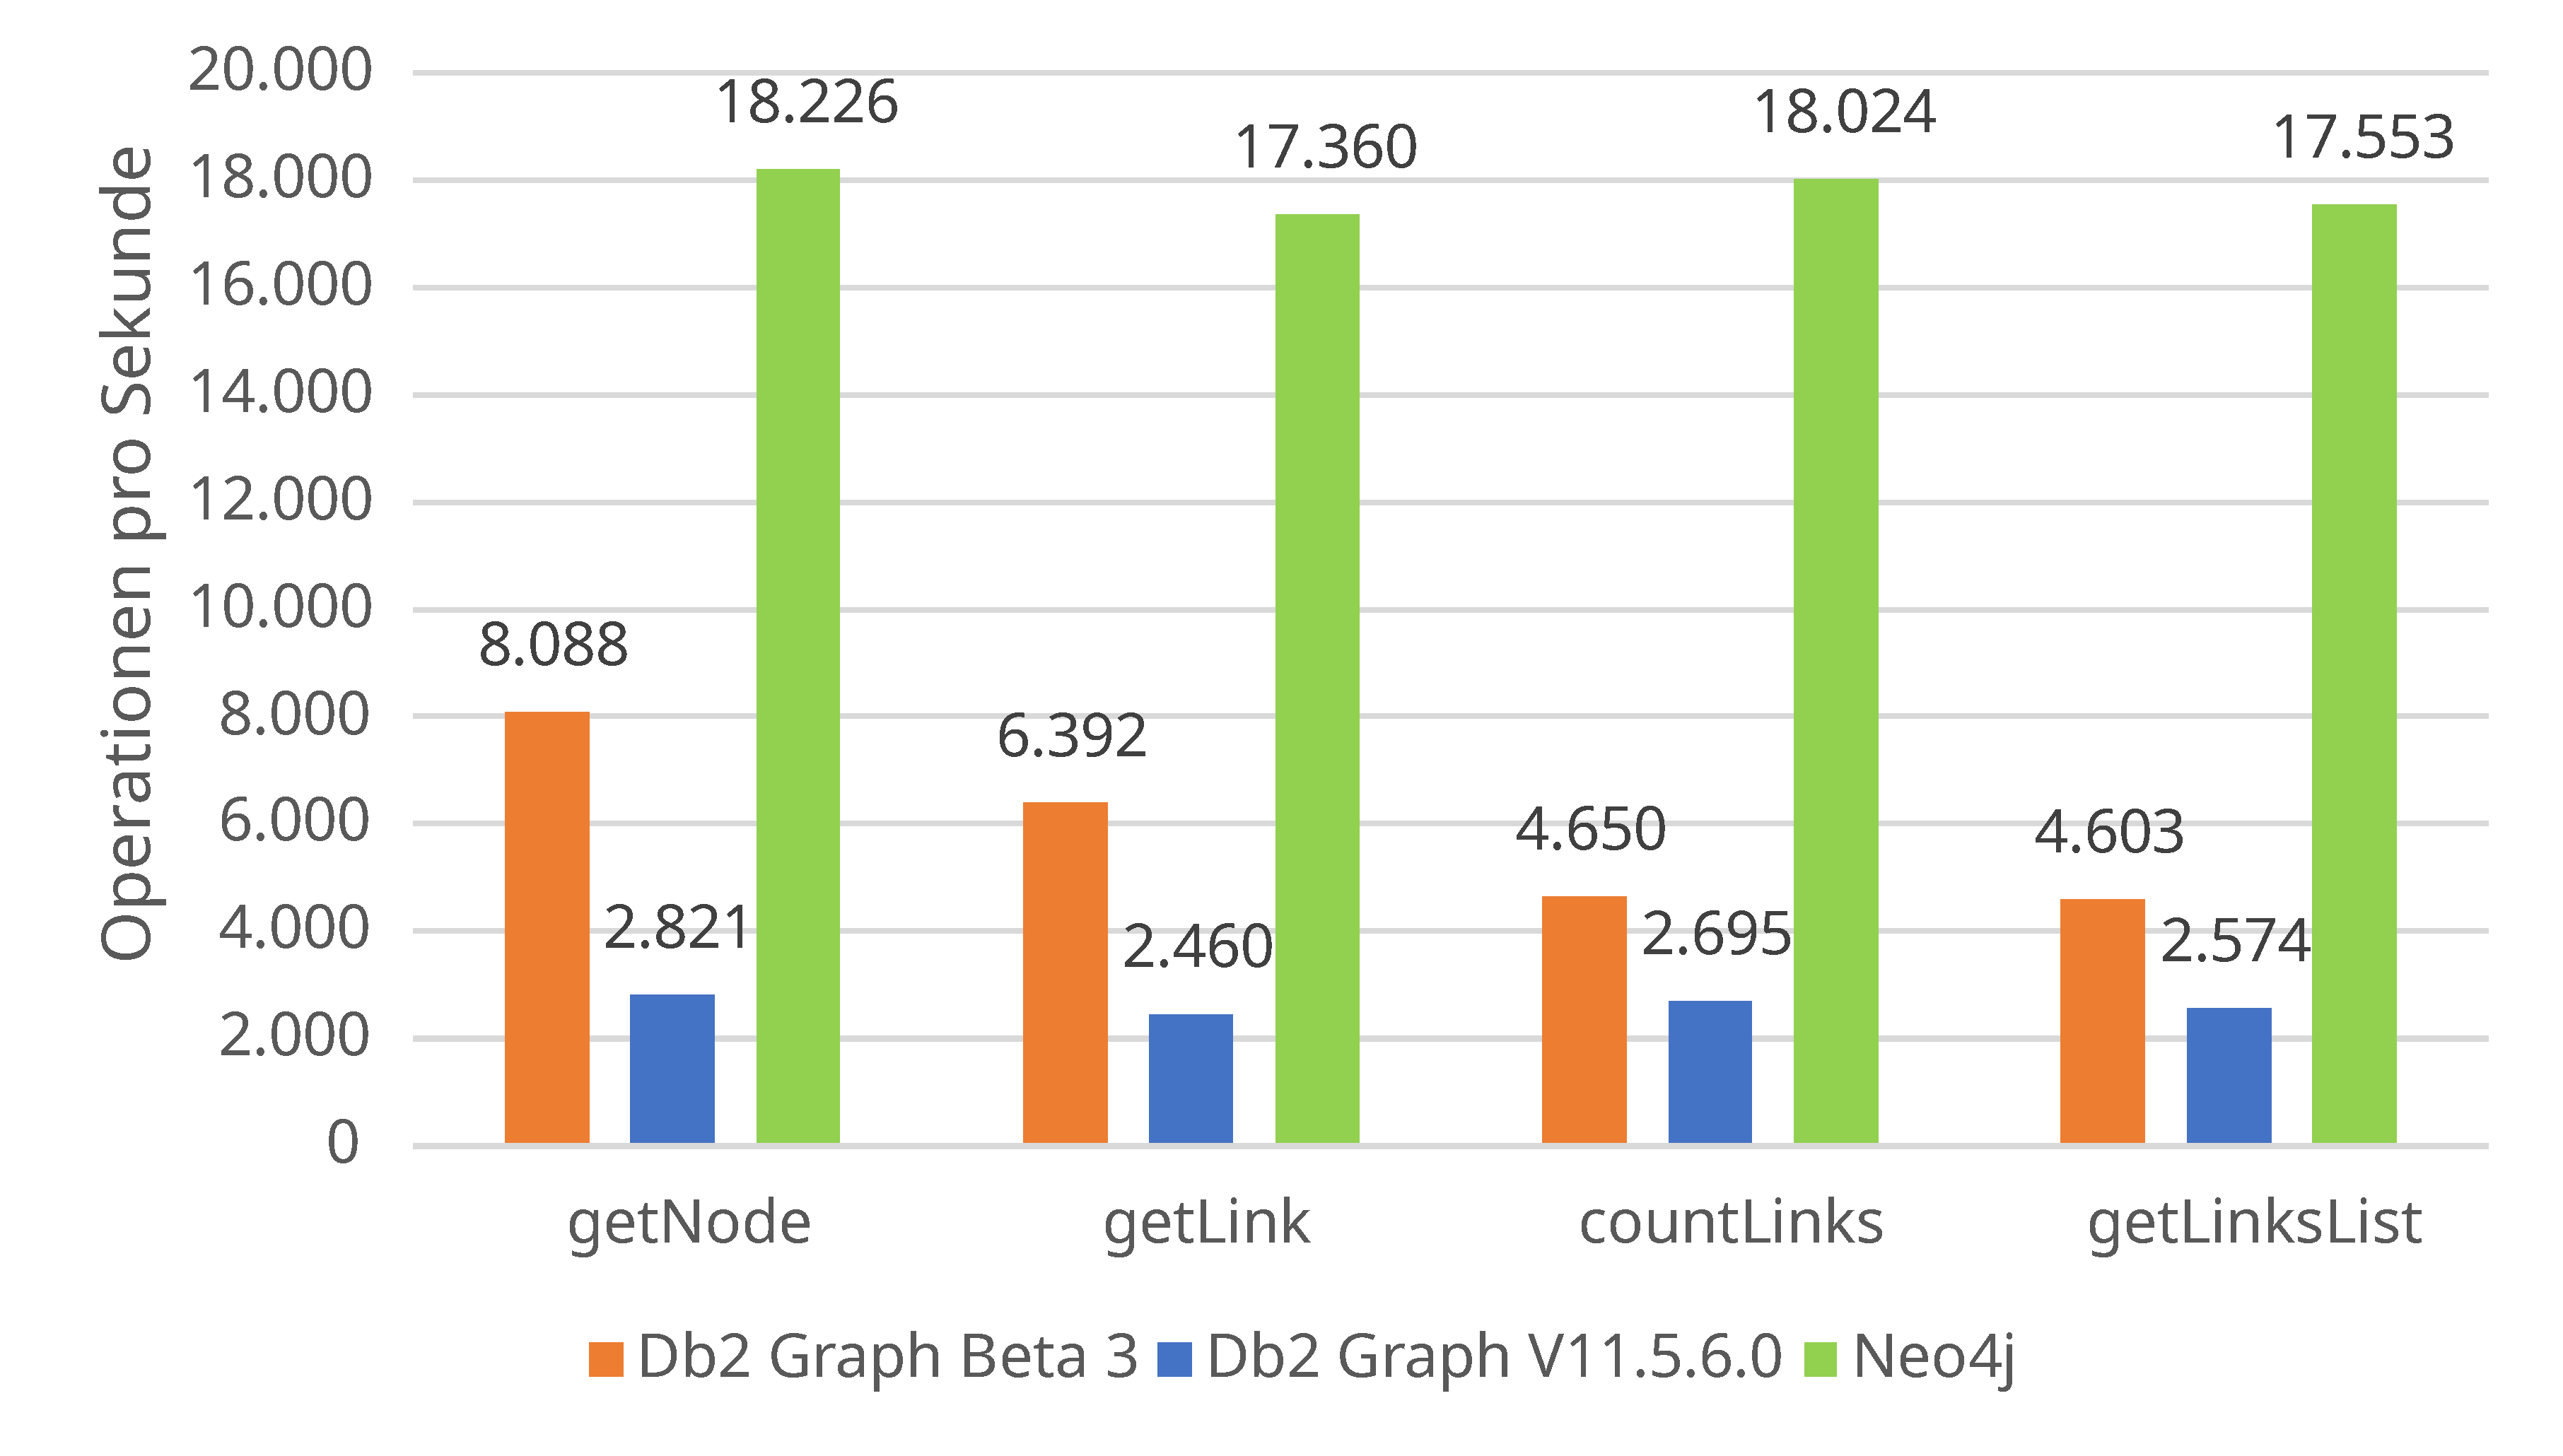
\includegraphics[width=\textwidth]{images/diagramme/linkbench_10m_const_durchsatz.pdf}
    \caption{Ergebnisse Durchsatz Linkbench-10M-Const}
    \label{fig:durchsatz:linkbench_10m_const}
\end{figure}

\section{Linkbench-100M-Const}
\label{ergebnisse:100m_const}
Im Rahmen dieses Abschnitts werden die Latenz- und Durchsatzergebnisse der Messreihe \nameref{ergebnisse:100m_const} aufgeführt und mit den Ergebnissen der Messreihe \nameref{ergebnisse:10m_const} verglichen. Schließlich handelt es sich hierbei um zwei Messreihen, die sich lediglich in der Größe des Datensatzes unterscheiden. Diese Messreihe verfügt hierbei um einen Datensatz, der um den Faktor-10 größer ist als der, der im Rahmen der Reihe \nameref{ergebnisse:10m_const} herangezogen wird. 

\subsection{Latenz}
Werden die in \autoref{tab:latenz_100m_const:beta3}, \autoref{tab:latenz_100m_const:ga} und \autoref{tab:latenz_100m_const:neo4j} aufgeführten Werte, die die Latenzergebnisse für Db2 Graph Beta 3, Db2 Graph V11.5.6.0 und Neo4j beinhalten, miteinander verglichen, so ergibt sich einmal mehr das Bild, dass Neo4j die geringste Latenz aller drei gebenchmarkten Datenbanksysteme aufweist. Auf Platz zwei der Datenbanksysteme mit der geringsten Latenz für die Operationen folgt dabei wieder Db2 Graph Beta 3. Es weist hierbei im Durchschnitt eine halb bis ein Drittel so hohen Latenzwert wie Db2 Graph V11.5.6.0 auf.

\begin{table}[!ht]
\centering
\resizebox{\textwidth}{!}{
\begin{tabular}{l|r|r|r|r|r|r|r}
\hline
\rowcolor[HTML]{EFEFEF} 
\multicolumn{1}{c|}{\cellcolor[HTML]{EFEFEF}\textbf{Operation}} &
\multicolumn{1}{c|}{\cellcolor[HTML]{EFEFEF}\textbf{Mean}} &
\multicolumn{1}{c|}{\cellcolor[HTML]{EFEFEF}\textbf{p25}} &
\multicolumn{1}{c|}{\cellcolor[HTML]{EFEFEF}\textbf{p50}} &
\multicolumn{1}{c|}{\cellcolor[HTML]{EFEFEF}\textbf{p75}} &
\multicolumn{1}{c|}{\cellcolor[HTML]{EFEFEF}\textbf{p95}} &
\multicolumn{1}{c|}{\cellcolor[HTML]{EFEFEF}\textbf{p99}} &
\multicolumn{1}{c}{\cellcolor[HTML]{EFEFEF}\textbf{Max.}} \\ \hline
getNode & 6,34ms & {[}4,5{]}ms & {[}5,6{]}ms & {[}7,8{]}ms & {[}10,11{]}ms & {[}16,17{]}ms & 808,08ms \\
getLink & 8,22ms & {[}6,7{]}ms & {[}7,8{]}ms & {[}9,10{]}ms & {[}13,14{]}ms & {[}20,21{]}ms & 1.500,61ms \\
countLink & 10,95ms & {[}8,9{]}ms & {[}10,11{]}ms & {[}12,13{]}ms & {[}17,18{]}ms & {[}24,25{]}ms & 402,42ms \\
getLinkList & 11,24ms & {[}8,9{]}ms & {[}10,11{]}ms & {[}12,13{]}ms & {[}17,18{]}ms & {[}24,25{]}ms & 791,5ms \\ \hline
\end{tabular}
}
\caption{Latenz Linkbench-100M-Const Db2 Graph Beta 3}
\label{tab:latenz_100m_const:beta3}
\end{table}

\begin{table}[!ht]
\centering
\resizebox{\textwidth}{!}{
\begin{tabular}{l|r|r|r|r|r|r|r}
\hline
\rowcolor[HTML]{EFEFEF} 
\multicolumn{1}{c|}{\cellcolor[HTML]{EFEFEF}\textbf{Operation}} &
\multicolumn{1}{c|}{\cellcolor[HTML]{EFEFEF}\textbf{Mean}} &
\multicolumn{1}{c|}{\cellcolor[HTML]{EFEFEF}\textbf{p25}} &
\multicolumn{1}{c|}{\cellcolor[HTML]{EFEFEF}\textbf{p50}} &
\multicolumn{1}{c|}{\cellcolor[HTML]{EFEFEF}\textbf{p75}} &
\multicolumn{1}{c|}{\cellcolor[HTML]{EFEFEF}\textbf{p95}} &
\multicolumn{1}{c|}{\cellcolor[HTML]{EFEFEF}\textbf{p99}} &
\multicolumn{1}{c}{\cellcolor[HTML]{EFEFEF}\textbf{Max.}} \\ \hline
getNode & 17,88ms & {[}4,5{]}ms & {[}13,14{]}ms & {[}29,30{]}ms & {[}42,43{]}ms & {[}48,49{]}ms & 680,9ms \\
getLink & 20,71ms & {[}6,7{]}ms & {[}14,15{]}ms & {[}33,34{]}ms & {[}48,49{]}ms & {[}56,57{]}ms & 1.807,64ms \\
countLink & 18,92ms & {[}5,6{]}ms & {[}13,14{]}ms & {[}30,31{]}ms & {[}45,46{]}ms & {[}52,53{]}ms & 704,75ms \\
getLinkList & 19,67ms & {[}5,6{]}ms & {[}13,14{]}ms & {[}32,33{]}ms & {[}47,48{]}ms & {[}54,55{]}ms & 3.792,33ms \\ \hline
\end{tabular}
}
\caption{Latenz Linkbench-100M-Const Db2 Graph V11.5.6.0}
\label{tab:latenz_100m_const:ga}
\end{table}

\begin{table}[!ht]
\centering
\resizebox{\textwidth}{!}{
\begin{tabular}{l|r|r|r|r|r|r|r}
\hline
\rowcolor[HTML]{EFEFEF} 
\multicolumn{1}{c|}{\cellcolor[HTML]{EFEFEF}\textbf{Operation}} &
\multicolumn{1}{c|}{\cellcolor[HTML]{EFEFEF}\textbf{Mean}} &
\multicolumn{1}{c|}{\cellcolor[HTML]{EFEFEF}\textbf{p25}} &
\multicolumn{1}{c|}{\cellcolor[HTML]{EFEFEF}\textbf{p50}} &
\multicolumn{1}{c|}{\cellcolor[HTML]{EFEFEF}\textbf{p75}} &
\multicolumn{1}{c|}{\cellcolor[HTML]{EFEFEF}\textbf{p95}} &
\multicolumn{1}{c|}{\cellcolor[HTML]{EFEFEF}\textbf{p99}} &
\multicolumn{1}{c}{\cellcolor[HTML]{EFEFEF}\textbf{Max.}} \\ \hline
getNode & 2,85ms & {[}2,3{]}ms & {[}2,3{]}ms & {[}3,4{]}ms & {[}3,4{]}ms & {[}4,5{]}ms & 1.080,62ms \\
getLink & 2,99ms & {[}2,3{]}ms & {[}2,3{]}ms & {[}3,4{]}ms & {[}4,5{]}ms & {[}5,6{]}ms & 1.306,96ms \\
countLink & 2,84ms & {[}2,3{]}ms & {[}2,3{]}ms & {[}3,4{]}ms & {[}3,4{]}ms & {[}4,5{]}ms & 1.222,04ms \\
getLinkList & 2,93ms & {[}2,3{]}ms & {[}2,3{]}ms & {[}3,4{]}ms & {[}4,5{]}ms & {[}5,6{]}ms & 975,43ms \\ \hline
\end{tabular}
}
\caption{Latenz Linkbench-100M-Const Neo4j}
\label{tab:latenz_100m_const:neo4j}
\end{table}

Beim Vergleich der in diesem Abschnitt aufgeführten Latenzergebnisse, mit denen aus \nameref{ergebnisse:10m_const} die auf Basis eines kleineren Datensatzes erzielt werden, fällt auf, dass die durchschnittlichen Latenzen bei allen Datenbanksystemen geringfügig höher ausfallen, als bei \nameref{ergebnisse:10m_const}. 

Dieses Verhalten entspricht dabei allerdings den Erwartungen, da normalerweise immer davon ausgegangen werden sollte, dass die Beantwortung der Queries auf Basis eines größeren Datensatzes mehr Zeit benötigt als bei einem kleinen Datensatz. Schließlich steigt hierbei der Verarbeitungsaufwand für die Datenbanksysteme. 

Der Unterschied zwischen den Messreihen fällt hier sogar kleiner aus als erwartet. Dies lässt sich vermutlich auf den großen Bufferpool oder Page-Cache der gebenchmarkten Datenbanksysteme zurückführen. So sollten sowohl der Linkbench-10M als auch der Linkbench-100M Datensatz komplett in den Bufferpool oder den Page-Cache von Db2 und Neo4j passen.

\subsection{Durchsatz}
Die im Rahmen dieser Messreihe erzielten Durchsatzwerte (\autoref{fig:durchsatz:linkbench_100m_const}) unterstreichen auch bei dieser Messreihe die bei den Latenzwerten beobachteten Sachverhalte. Auch hier weist Db2 Graph V11.5.6.0 den geringsten Wert auf, Neo4j hingegen wieder einmal den höchsten. Auch bleiben die Durchsatzwerte alle geringfügig unterhalb der Werte aus \autoref{fig:durchsatz:linkbench_10m_const}, die auf Basis des kleineren Datensatzes aber gleich verteilten Datensatzes ermittelt werden. 

\begin{figure}[!ht]
    \centering
    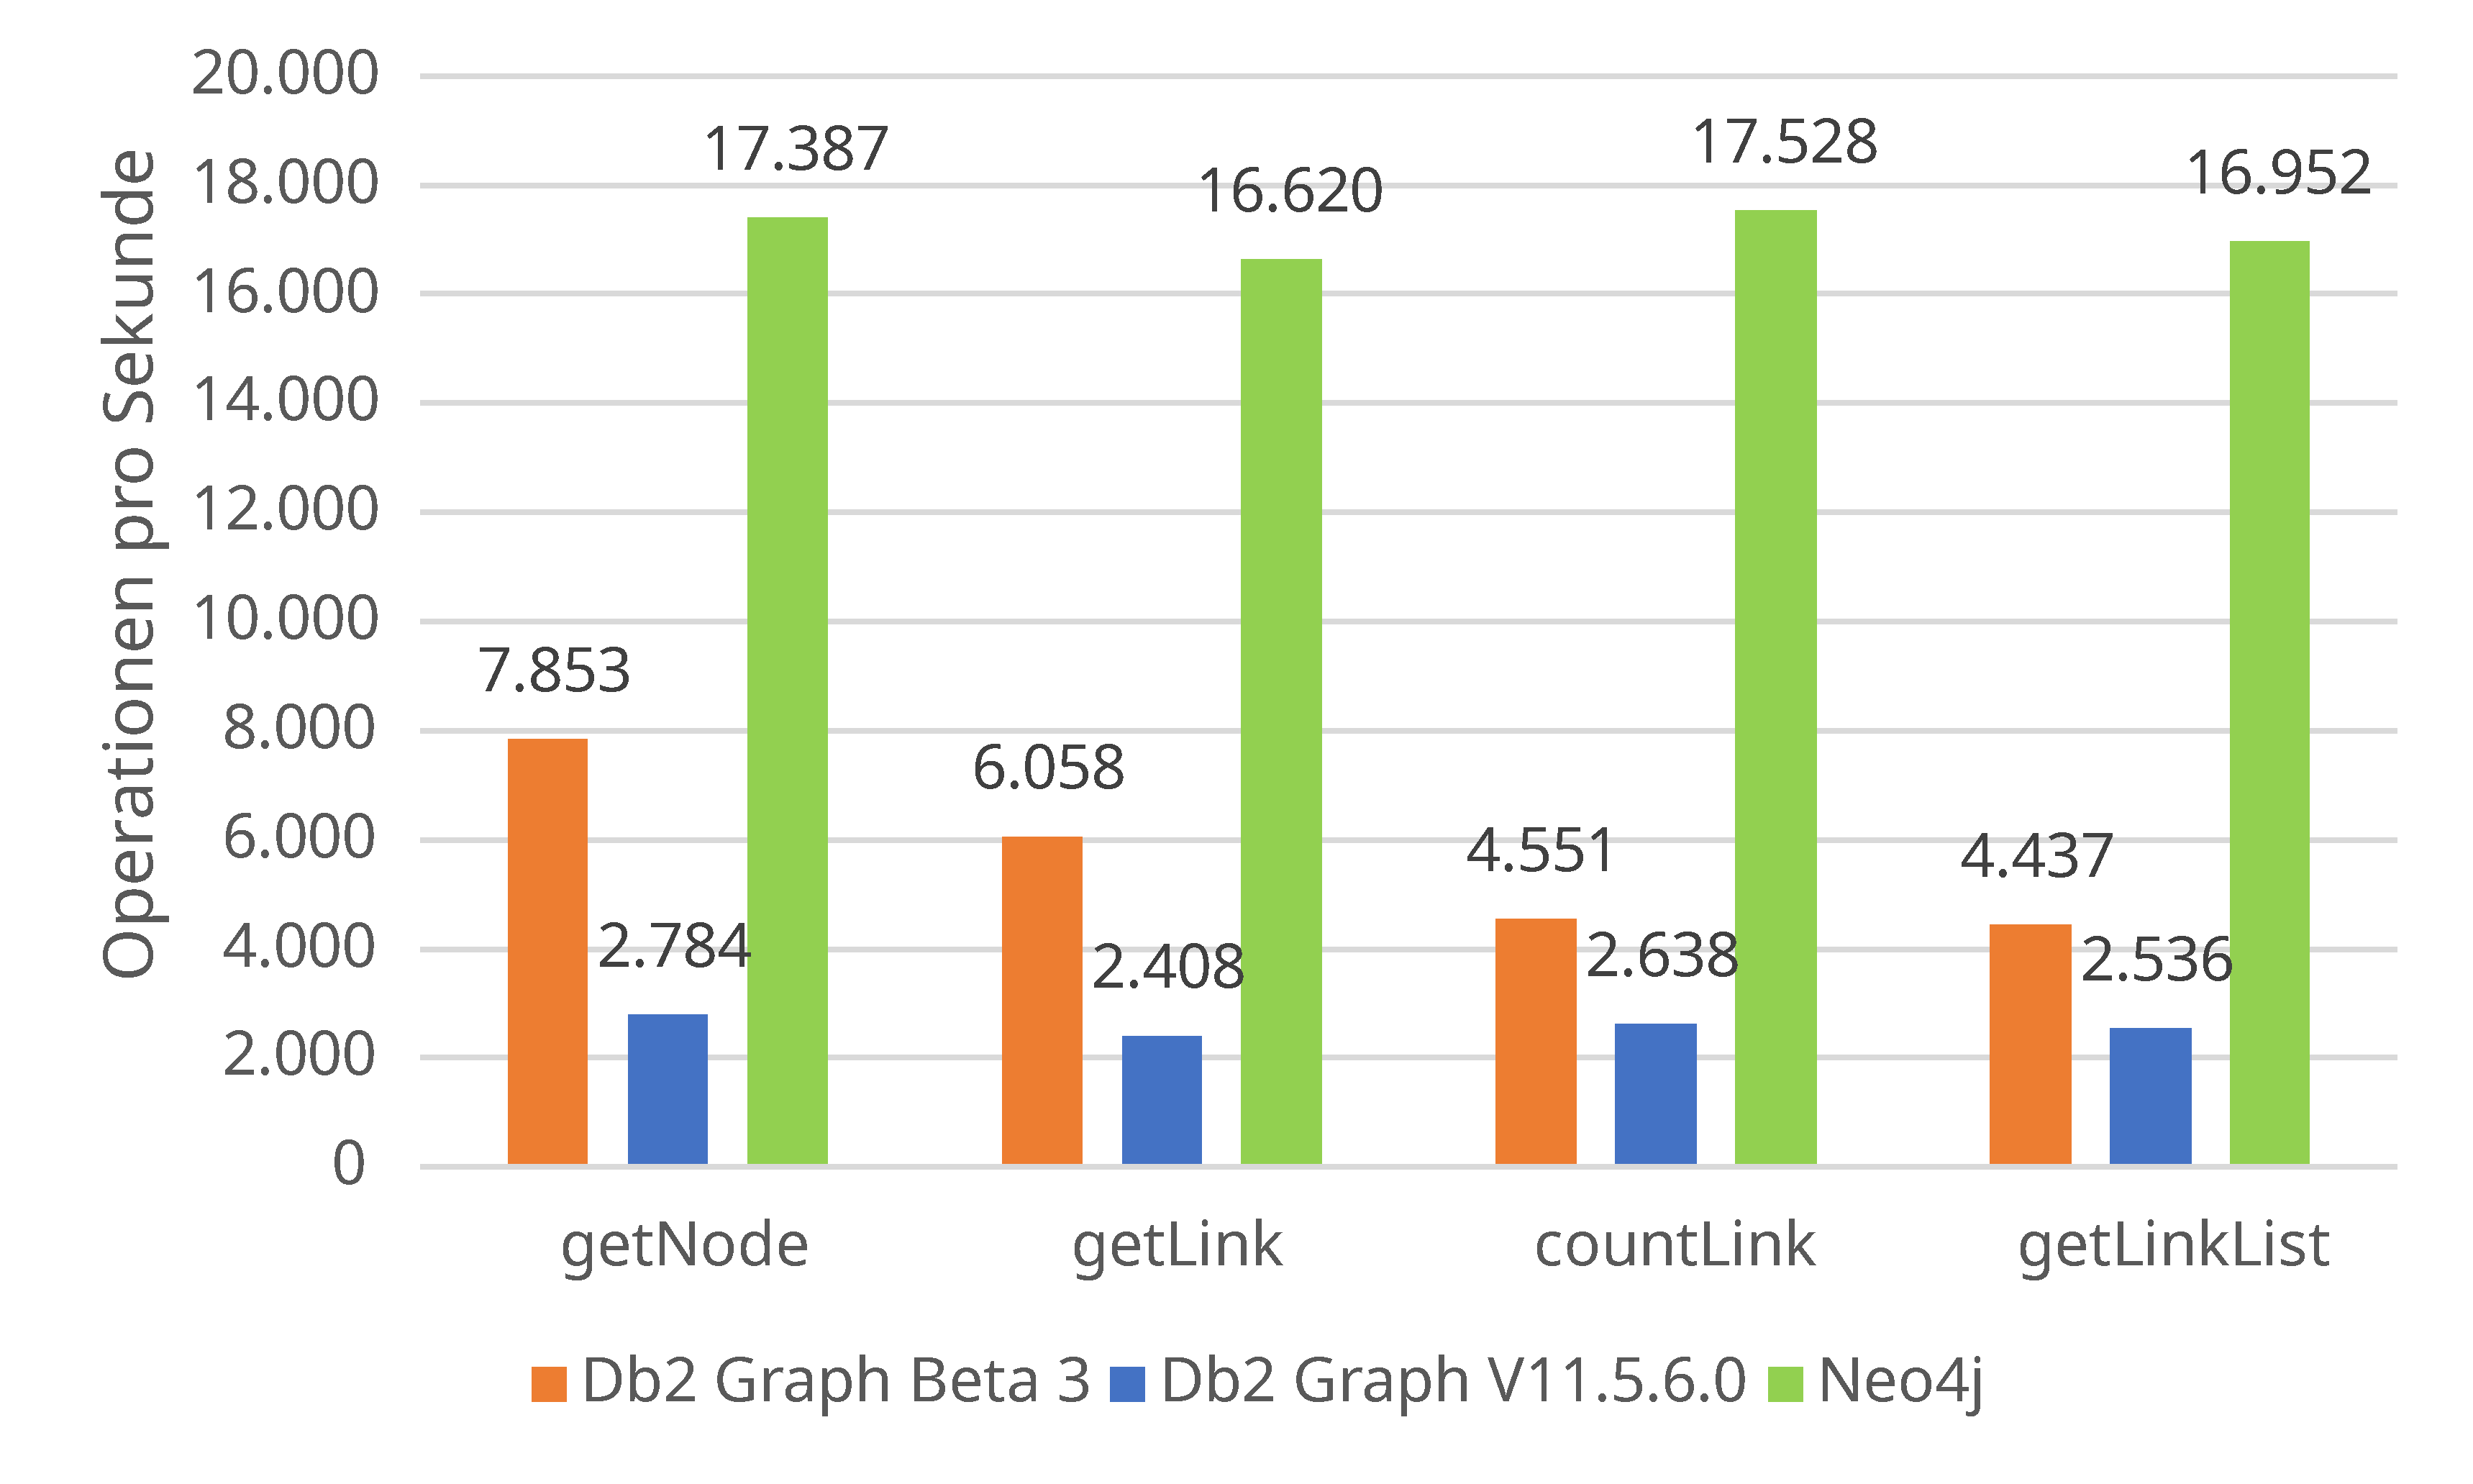
\includegraphics[width=\textwidth]{images/diagramme/linkbench_100m_const_durchsatz.pdf}
    \caption{Ergebnisse Durchsatz Linkbench-100M-Const}
    \label{fig:durchsatz:linkbench_100m_const}
\end{figure}

\section{Linkbench-10M-Real}
\label{ergebnisse:10m_real}
In diesem Abschnitt werden die Ergebnisse für die Messreihe \nameref{ergebnisse:10m_real} dargestellt und untersucht. Hierbei handelt es sich um die ersten Messergebnisse die für einen (kleinen) real verteilten Datensatz erzielt werden. So beinhalten die hier aufgeführten Messergebnisse sowohl Latenz- als auch Durchsatzwerte für die \texttt{getLinkList}-Operation mit jeweils verschieden hohen Ergebnismenge. Das Datenbanksystem Db2 Graph Beta 3 spielt dabei in den Messungen keine Rolle.

\subsection{Latenz}
Bei der Analyse der Latenzwerte von Db2 Graph V11.5.6.0 (\autoref{tab:latenz_10m_real:ga} und \autoref{tab:latenz_10m_real:ga:gll}) und Neo4j (\autoref{tab:latenz_10m_real:neo4j} und \autoref{tab:latenz_10m_real:neo4j:gll}) bietet sich ein ähnlicher Anblick, wie bei den konstant verteilten Datensätzen. Neo4j weist weitaus geringere Latenzergebnisse auf als Db2 Graph V11.5.6.0. 

In Bezug zu den Latenzwerten für die \texttt{getLinkList}-Operation mit jeweils unterschiedlichen Grenzen für die Ergebnismenge fällt auf, dass die Durchschnittslatenzen von Db2 Graph und Neo4j zwischen den Messungen mit einer maximalen Ergebnismenge von 100 und 100.000 nahezu verdoppeln. Somit kann daran abgeleitet werden, dass hier die Performance der Datenbanksysteme mit einer steigenden Grenze für die Ergebnismenge sinkt.

\begin{table}[!ht]
\centering
\resizebox{\textwidth}{!}{
\begin{tabular}{l|r|r|r|r|r|r|r}
\hline
\rowcolor[HTML]{EFEFEF} 
\multicolumn{1}{c|}{\cellcolor[HTML]{EFEFEF}\textbf{Operation}} &
\multicolumn{1}{c|}{\cellcolor[HTML]{EFEFEF}\textbf{Mean}} &
\multicolumn{1}{c|}{\cellcolor[HTML]{EFEFEF}\textbf{p25}} &
\multicolumn{1}{c|}{\cellcolor[HTML]{EFEFEF}\textbf{p50}} &
\multicolumn{1}{c|}{\cellcolor[HTML]{EFEFEF}\textbf{p75}} &
\multicolumn{1}{c|}{\cellcolor[HTML]{EFEFEF}\textbf{p95}} &
\multicolumn{1}{c|}{\cellcolor[HTML]{EFEFEF}\textbf{p99}} &
\multicolumn{1}{c}{\cellcolor[HTML]{EFEFEF}\textbf{Max.}} \\ \hline
getNode & 17,88ms & {[}4,5{]}ms & {[}13,14{]}ms & {[}29,30{]}ms & {[}42,43{]}ms & {[}49,50{]}ms & 293,64ms \\
getLink & 20,47ms & {[}6,7{]}ms & {[}14,15{]}ms & {[}33,34{]}ms & {[}49,50{]}ms & {[}57,58{]}ms & 356,93ms \\
countLink & 18,32ms & {[}5,6{]}ms & {[}12,13{]}ms & {[}30,31{]}ms & {[}44,45{]}ms & {[}51,52{]}ms & 277,05ms \\ \hline
\end{tabular}
}
\caption{Latenz Linkbench-10M-Real Db2 Graph V11.5.6.0}
\label{tab:latenz_10m_real:ga}
\end{table}    

\begin{table}[!ht]
\centering
\resizebox{\textwidth}{!}{
\begin{tabular}{r|r|r|r|r|r|r|r}
\hline
\rowcolor[HTML]{EFEFEF} 
\multicolumn{1}{c|}{\cellcolor[HTML]{EFEFEF}\textbf{Mean}} &
\multicolumn{1}{c|}{\cellcolor[HTML]{EFEFEF}\textbf{p25}} &
\multicolumn{1}{c|}{\cellcolor[HTML]{EFEFEF}\textbf{p50}} &
\multicolumn{1}{c|}{\cellcolor[HTML]{EFEFEF}\textbf{p75}} &
\multicolumn{1}{c|}{\cellcolor[HTML]{EFEFEF}\textbf{p95}} &
\multicolumn{1}{c|}{\cellcolor[HTML]{EFEFEF}\textbf{p99}} &
\multicolumn{1}{c|}{\cellcolor[HTML]{EFEFEF}\textbf{Max.}} &
\multicolumn{1}{c}{\cellcolor[HTML]{EFEFEF}\textbf{Limit}} \\ \hline
19,64ms & {[}5,6{]}ms & {[}13,14{]}ms & {[}32,33{]}ms & {[}47,48{]}ms & {[}55,56{]}ms & 401,99ms & 100\\
20,12ms & {[}5,6{]}ms & {[}14,15{]}ms & {[}32,33{]}ms & {[}48,49{]}ms & {[}57,58{]}ms & 442,84ms & 1.000\\
22,37ms & {[}5,6{]}ms & {[}15,16{]}ms & {[}35,36{]}ms & {[}53,54{]}ms & {[}68,69{]}ms & 776,83ms & 10.000\\
34,00ms & {[}6,7{]}ms & {[}20,21{]}ms & {[}44,45{]}ms & {[}82,83{]}ms & {[}100,200{]}ms & 3.125,17ms & 100.000\\ \hline
\end{tabular}
}
\caption{Latenz Linkbench-10M-Real Db2 Graph V11.5.6.0 getLinkList}
\label{tab:latenz_10m_real:ga:gll}
\end{table}

\begin{table}[!ht]
\centering
\resizebox{\textwidth}{!}{
\begin{tabular}{l|r|r|r|r|r|r|r}
\hline
\rowcolor[HTML]{EFEFEF} 
\multicolumn{1}{c|}{\cellcolor[HTML]{EFEFEF}\textbf{Operation}} &
\multicolumn{1}{c|}{\cellcolor[HTML]{EFEFEF}\textbf{Mean}} &
\multicolumn{1}{c|}{\cellcolor[HTML]{EFEFEF}\textbf{p25}} &
\multicolumn{1}{c|}{\cellcolor[HTML]{EFEFEF}\textbf{p50}} &
\multicolumn{1}{c|}{\cellcolor[HTML]{EFEFEF}\textbf{p75}} &
\multicolumn{1}{c|}{\cellcolor[HTML]{EFEFEF}\textbf{p95}} &
\multicolumn{1}{c|}{\cellcolor[HTML]{EFEFEF}\textbf{p99}} &
\multicolumn{1}{c}{\cellcolor[HTML]{EFEFEF}\textbf{Max.}} \\ \hline
getNode & 2,89ms & {[}2,3{]}ms & {[}2,3{]}ms & {[}3,4{]}ms & {[}3,4{]}ms & {[}5,6{]}ms & 1.073,54ms \\
getLink & 3,30ms & {[}2,3{]}ms & {[}2,3{]}ms & {[}3,4{]}ms & {[}5,6{]}ms & {[}9,10{]}ms & 2.433,82ms \\
countLink & 3,05ms & {[}2,3{]}ms & {[}2,3{]}ms & {[}3,4{]}ms & {[}4,5{]}ms & {[}8,9{]}ms & 1.381,42ms \\ \hline
\end{tabular}
}
\caption{Latenz Linkbench-10M-Real Neo4j}
\label{tab:latenz_10m_real:neo4j}
\end{table}

\begin{table}[!ht]
\centering
\resizebox{\textwidth}{!}{
\begin{tabular}{l|r|r|r|r|r|r|r}
\hline
\rowcolor[HTML]{EFEFEF} 
\multicolumn{1}{c|}{\cellcolor[HTML]{EFEFEF}\textbf{Operation}} &
\multicolumn{1}{c|}{\cellcolor[HTML]{EFEFEF}\textbf{Mean}} &
\multicolumn{1}{c|}{\cellcolor[HTML]{EFEFEF}\textbf{p25}} &
\multicolumn{1}{c|}{\cellcolor[HTML]{EFEFEF}\textbf{p50}} &
\multicolumn{1}{c|}{\cellcolor[HTML]{EFEFEF}\textbf{p75}} &
\multicolumn{1}{c|}{\cellcolor[HTML]{EFEFEF}\textbf{p95}} &
\multicolumn{1}{c|}{\cellcolor[HTML]{EFEFEF}\textbf{p99}} &
\multicolumn{1}{c}{\cellcolor[HTML]{EFEFEF}\textbf{Max.}} \\ \hline
getLinkList & 3,08ms & {[}2,3{]}ms & {[}2,3{]}ms & {[}3,4{]}ms & {[}4,5{]}ms & {[}8,9{]}ms & 1.021,83ms \\
getLinkList & 3,42ms & {[}2,3{]}ms & {[}2,3{]}ms & {[}3,4{]}ms & {[}6,7{]}ms & {[}11,12{]}ms & 982,84ms \\
getLinkList & 4,38ms & {[}2,3{]}ms & {[}3,4{]}ms & {[}4,5{]}ms & {[}8,9{]}ms & {[}16,17{]}ms & 1.041,73ms \\
getLinkList & 5,46ms & {[}2,3{]}ms & {[}2,3{]}ms & {[}4,5{]}ms & {[}8,9{]}ms & {[}21,22{]}ms & 1.855,68ms \\ \hline
\end{tabular}
}
\caption{Latenz Linkbench-10M-Real Neo4j getLinkList}
\label{tab:latenz_10m_real:neo4j:gll}
\end{table}

\subsection{Durchsatz}
Die im Kontext dieser Messreihe ermittelten Durchsatzwerte (\autoref{fig:durchsatz:linkbench_10m_real} und \autoref{fig:durchsatz:linkbench_10m_real:rl}) bestätigen die bereits bei den Latenzen entdeckten Phänomene. So weist Neo4j durch den höheren Durchsatz bei allen gebenchmarkten Operationen eine bessere Performance als Db2 Graph V11.5.6.0 auf. 

Analog zu der Verdoppelung der Latenzwerte halbieren sich auch bei beiden Datenbanksystemen die Durchsatzergebnisse der \texttt{getLinkList}-Operation zwischen den Messungen mit einem Range-Limit von 100 und 100.000.

\begin{figure}[!ht]
    \centering
    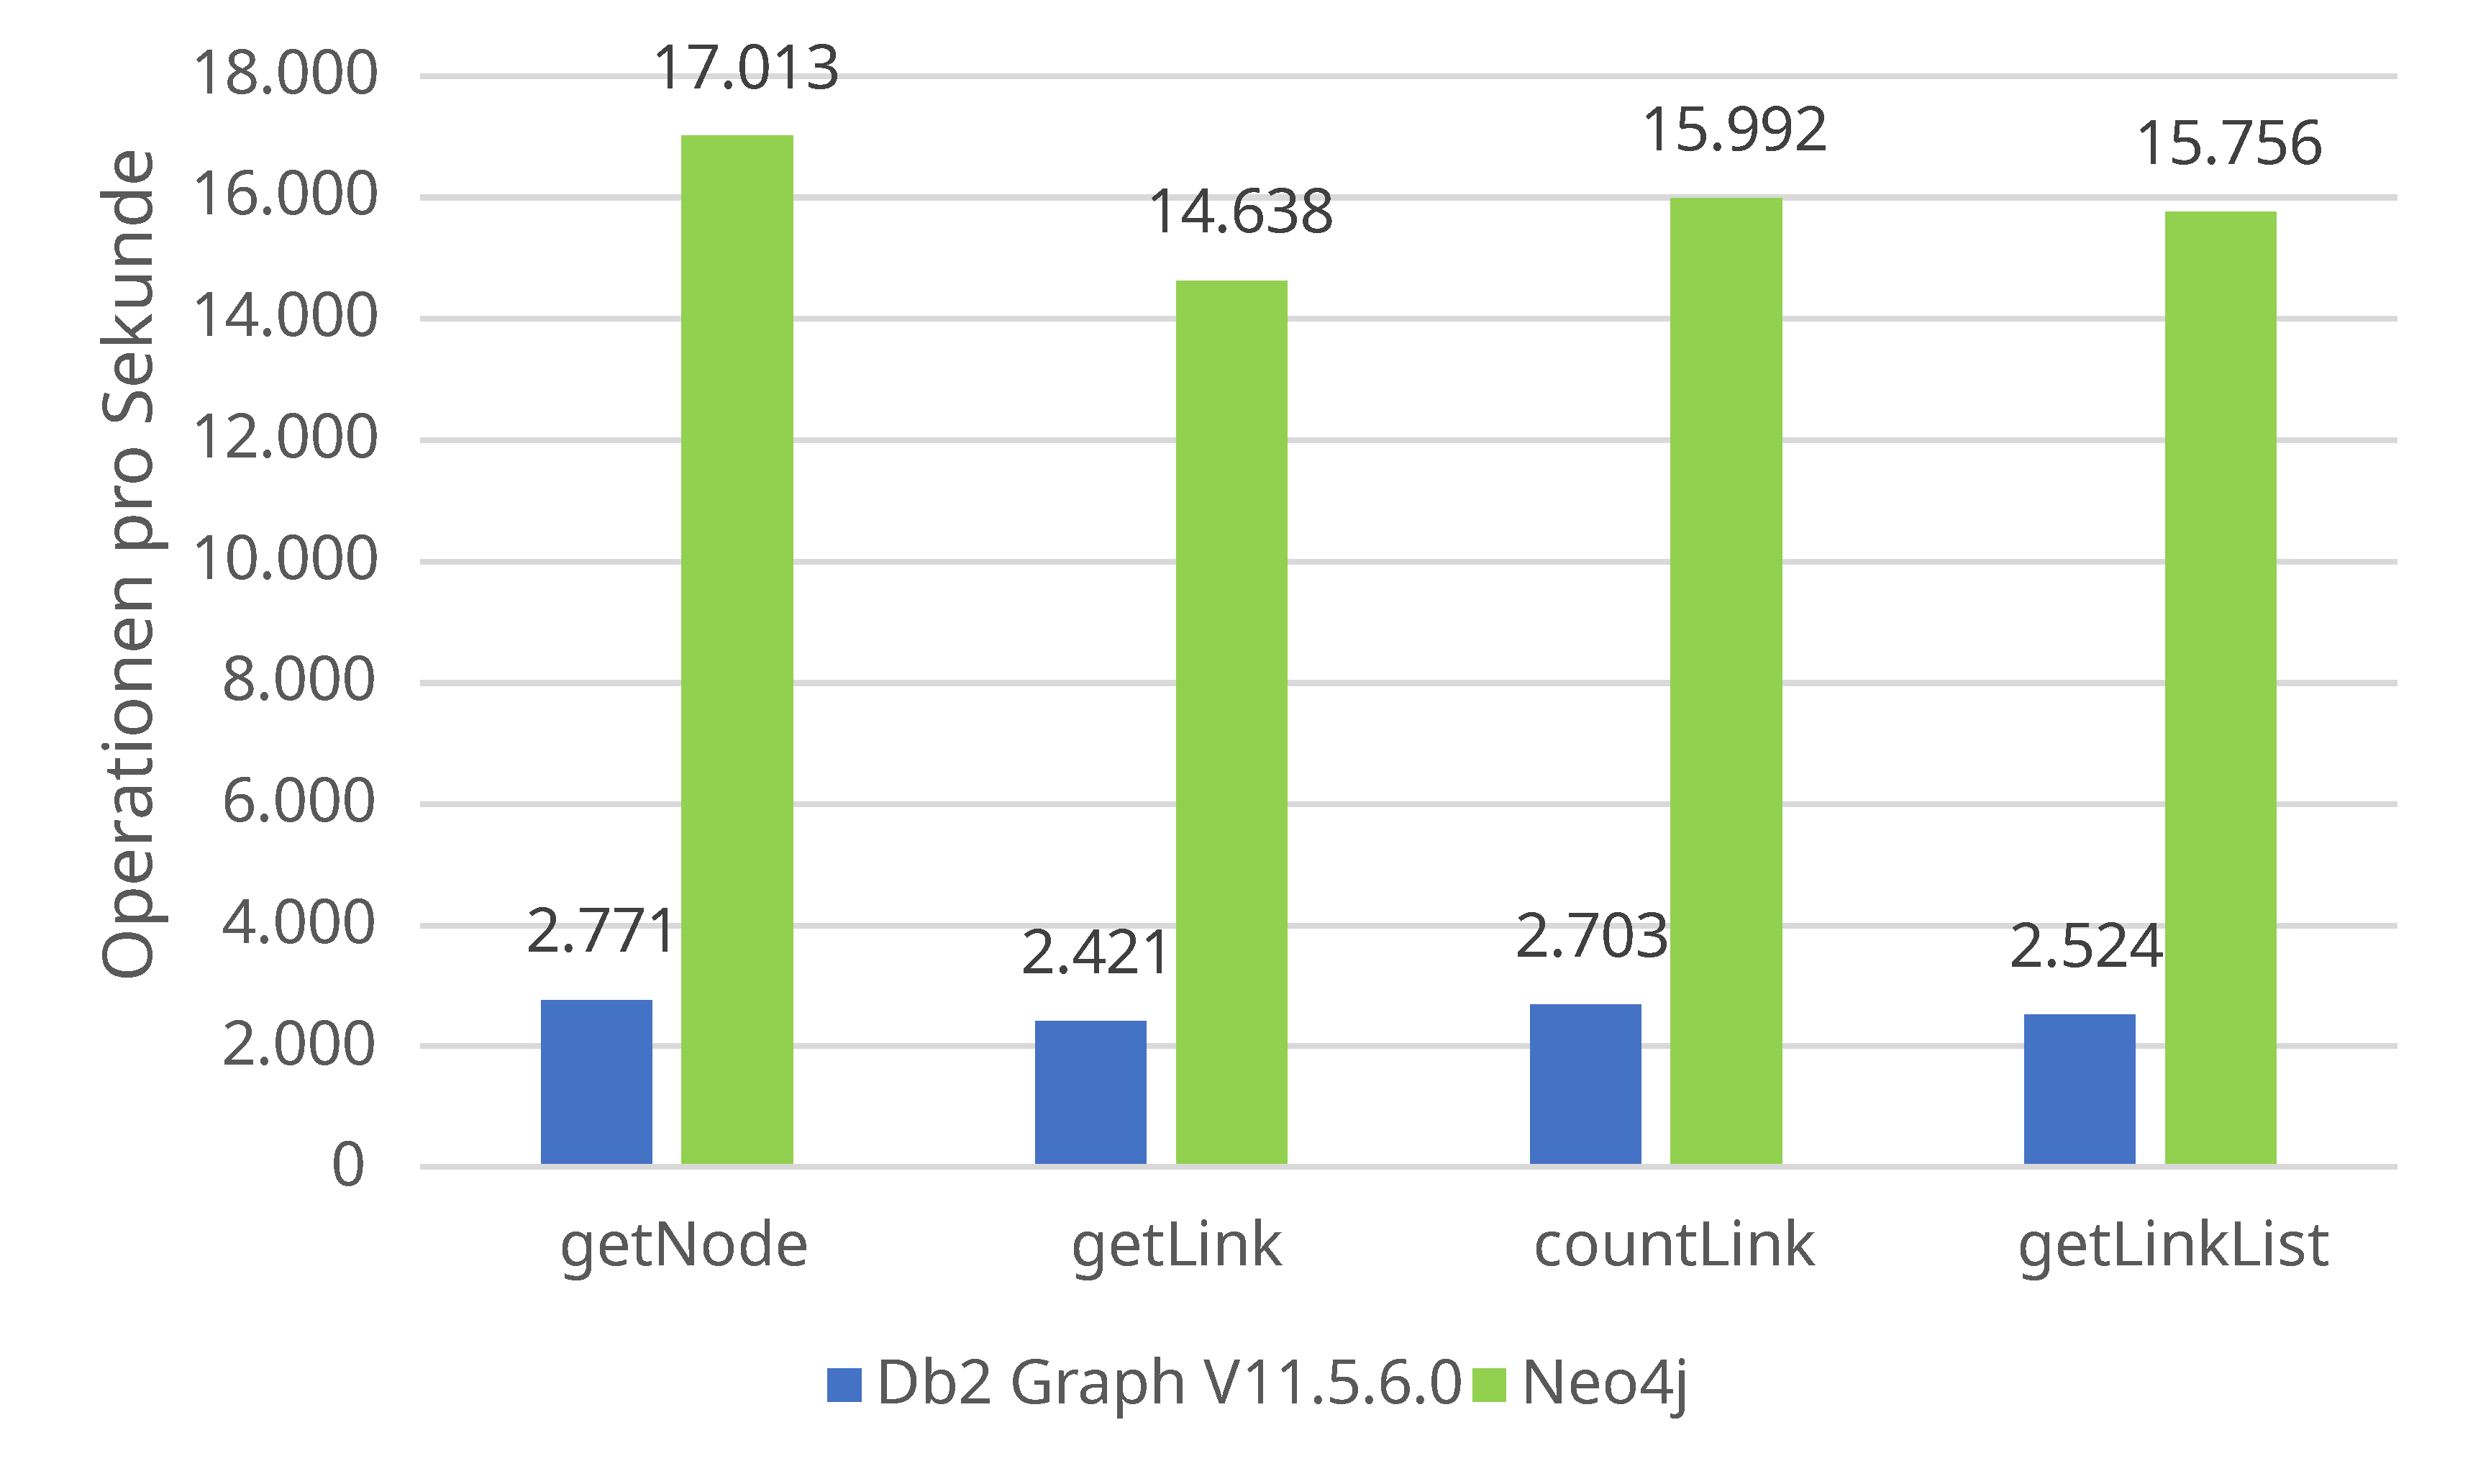
\includegraphics[width=\textwidth]{images/diagramme/linkbench_10m_real_durchsatz.pdf}
    \caption{Ergebnisse Durchsatz Linkbench-10M-Real}
    \label{fig:durchsatz:linkbench_10m_real}
    \vspace{1em}
    \textit{Die bei getLinkList abgebildeten Werte repräsentieren die Ergebnisse, die mit einer Begrenzung der Ergebnismenge auf maximal 100 Elemente erzielt werden.}
\end{figure}

\begin{figure}[!ht]
    \centering
    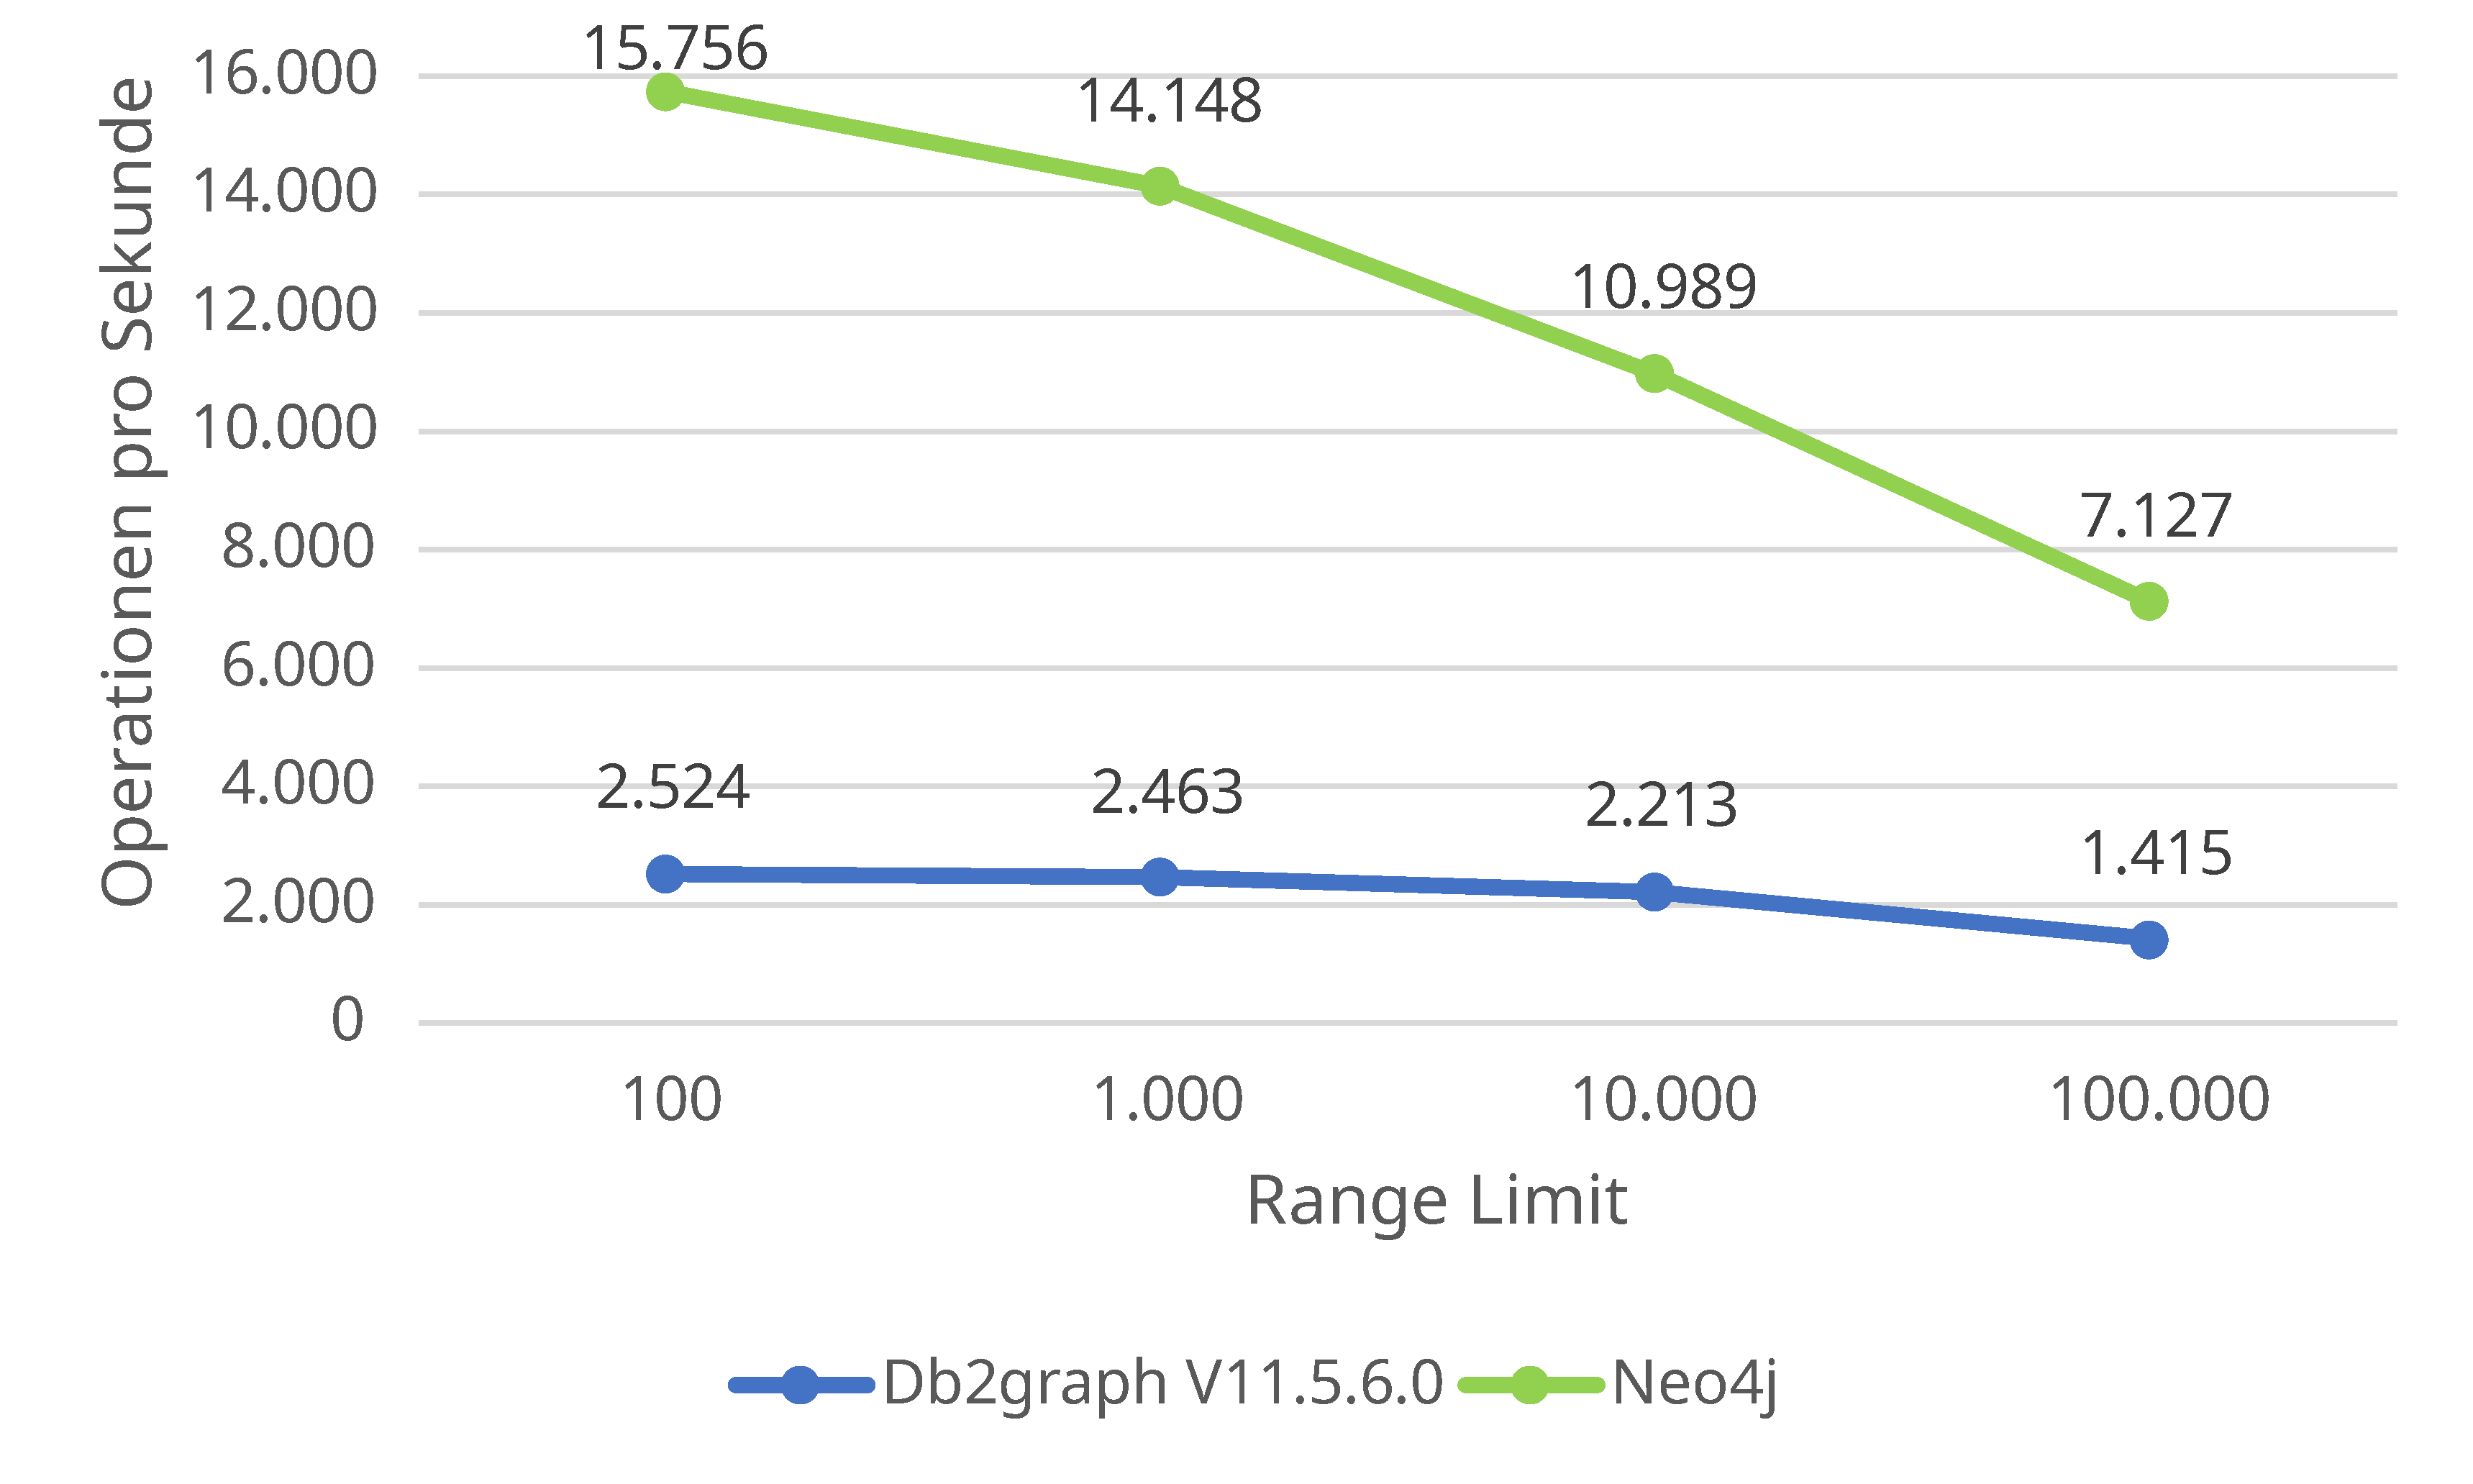
\includegraphics[width=\textwidth]{images/diagramme/limit_absolute_durchsatz_real_10m.pdf}
    \caption{Ergebnisse Durchsatz Linkbench-10M-Real getLinkList}
    \label{fig:durchsatz:linkbench_10m_real:rl}
\end{figure}

\section{Linkbench-100M-Real}
\label{ergebnisse:100m_real}
Im Rahmen dieses Abschnitts werden die Latenz- und Durchsatzergebnisse für Db2 Graph V11.5.6.0 und Neo4j aufgeführt. Alle Messungen deren Ergebnisse hier zur Schau gestellt werden, werden alle auf Basis eines größeren real verteilten Datensatzes erzielt. So umfasst der Datensatz dieser Messreihe (\nameref{ergebnisse:100m_real}) die zehnfache Anzahl an Knoten und Kanten wie der Datensatz der Messreihe \nameref{ergebnisse:10m_real}. Wie bereits bei \nameref{ergebnisse:10m_real} spielt Db2 Graph Beta 3 auch im Kontext dieses Abschnitts keine Rolle. Darüber hinaus existieren ebenfalls mehrere Messergebnisse für die \texttt{getLinkList}-Operation mit einer variierenden Beschränkung der Ergebnismenge.

\subsection{Latenz}
Bei der Untersuchung der Latenzwerte von Db2 Graph V11.5.6.0 (\autoref{tab:latenz_100m_real:ga} und \autoref{tab:latenz_100m_real:ga:gll}) und Neo4j (\autoref{tab:latenz_100m_real:neo4j} und \autoref{tab:latenz_100m_real:neo4j:gll}) fällt auf, dass Neo4j wieder deutlich niedrigere Durchschnittslatenzen aufweist als Db2 Graph V11.5.6.0. 

Die Messergebnisse für die Latenzen beider Datenbanksysteme ähneln dabei denen des kleineren real verteilten Datensatzes aus \nameref{ergebnisse:10m_real}. Dieses Verhalten könnte sich wie bereits bei den konstant verteilten Datensätzen basierten Messreihen damit erklären, dass Db2 und Neo4j beiden um einen Bufferpool und Page-Cache verfügen, in alle Datensätze vollständig geladen werden können, egal ob Linkbench-10M oder Linkbench-100M.

Bei der Analyse der durchschnittlichen Latenzen der \texttt{getLinkList}-Operationen mit variierender Ergebnismenge kann hierbei identifiziert werden, dass die Db2 Graph V11.5.6.0  (\autoref{tab:latenz_10m_real:ga}) und Neo4j Werte beide bei der steigenden Beschränkung der Ergebnismenge deutlich erhöhen. Bei Neo4j verdoppelt sich hierbei die durchschnittliche Latenz sogar, während dies bei Db2 Graph V11.5.6.0 nicht der Fall ist.

\begin{table}[!ht]
\centering
\resizebox{\textwidth}{!}{
\begin{tabular}{l|r|r|r|r|r|r|r}
\hline
\rowcolor[HTML]{EFEFEF} 
\multicolumn{1}{c|}{\cellcolor[HTML]{EFEFEF}\textbf{Operation}} &
\multicolumn{1}{c|}{\cellcolor[HTML]{EFEFEF}\textbf{Mean}} &
\multicolumn{1}{c|}{\cellcolor[HTML]{EFEFEF}\textbf{p25}} &
\multicolumn{1}{c|}{\cellcolor[HTML]{EFEFEF}\textbf{p50}} &
\multicolumn{1}{c|}{\cellcolor[HTML]{EFEFEF}\textbf{p75}} &
\multicolumn{1}{c|}{\cellcolor[HTML]{EFEFEF}\textbf{p95}} &
\multicolumn{1}{c|}{\cellcolor[HTML]{EFEFEF}\textbf{p99}} &
\multicolumn{1}{c}{\cellcolor[HTML]{EFEFEF}\textbf{Max.}} \\ \hline
getNode & 17,91ms & {[}5,6{]}ms & {[}13,14{]}ms & {[}29,30{]}ms & {[}42,43{]}ms & {[}49,50{]}ms & 520,53ms \\
getLink & 20,91ms & {[}7,8{]}ms & {[}14,15{]}ms & {[}33,34{]}ms & {[}49,50{]}ms & {[}57,58{]}ms & 811,52ms \\
countLink & 18,88ms & {[}5,6{]}ms & {[}13,14{]}ms & {[}30,31{]}ms & {[}45,46{]}ms & {[}52,53{]}ms & 661,18ms \\ \hline
\end{tabular}
}
\caption{Latenz Linkbench-100-Real Db2 Graph V11.5.6.0}
\label{tab:latenz_100m_real:ga}
\end{table}

\begin{table}[!ht]
\centering
\resizebox{\textwidth}{!}{
\begin{tabular}{r|r|r|r|r|r|r|r}
\hline
\rowcolor[HTML]{EFEFEF} 
\multicolumn{1}{c|}{\cellcolor[HTML]{EFEFEF}\textbf{Mean}} &
\multicolumn{1}{c|}{\cellcolor[HTML]{EFEFEF}\textbf{p25}} &
\multicolumn{1}{c|}{\cellcolor[HTML]{EFEFEF}\textbf{p50}} &
\multicolumn{1}{c|}{\cellcolor[HTML]{EFEFEF}\textbf{p75}} &
\multicolumn{1}{c|}{\cellcolor[HTML]{EFEFEF}\textbf{p95}} &
\multicolumn{1}{c|}{\cellcolor[HTML]{EFEFEF}\textbf{p99}} &
\multicolumn{1}{c|}{\cellcolor[HTML]{EFEFEF}\textbf{Max.}} &
\multicolumn{1}{c}{\cellcolor[HTML]{EFEFEF}\textbf{Limit}} \\ \hline
20,06ms & {[}6,7{]}ms & {[}14,15{]}ms & {[}32,33{]}ms & {[}47,48{]}ms & {[}54,55{]}ms & 502,66ms & 100\\
20,78ms & {[}6,7{]}ms & {[}14,15{]}ms & {[}33,34{]}ms & {[}49,50{]}ms & {[}58,59{]}ms & 2.003,24ms & 1.000\\
22,56ms & {[}6,7{]}ms & {[}15,16{]}ms & {[}35,36{]}ms & {[}53,54{]}ms & {[}67,68{]}ms & 2.553,64ms & 10.000\\
36,62ms & {[}7,8{]}ms & {[}21,22{]}ms & {[}46,47{]}ms & {[}89,90{]}ms & {[}100,200{]}ms & 4.351,98ms & 100.000\\ \hline
\end{tabular}
}
\caption{Latenz Linkbench-100M-Real Db2 Graph V11.5.6.0 getLinkList}
\label{tab:latenz_100m_real:ga:gll}
\end{table}

\begin{table}[!ht]
\centering
\resizebox{\textwidth}{!}{
\begin{tabular}{l|r|r|r|r|r|r|r}
\hline
\rowcolor[HTML]{EFEFEF} 
\multicolumn{1}{c|}{\cellcolor[HTML]{EFEFEF}\textbf{Operation}} &
\multicolumn{1}{c|}{\cellcolor[HTML]{EFEFEF}\textbf{Mean}} &
\multicolumn{1}{c|}{\cellcolor[HTML]{EFEFEF}\textbf{p25}} &
\multicolumn{1}{c|}{\cellcolor[HTML]{EFEFEF}\textbf{p50}} &
\multicolumn{1}{c|}{\cellcolor[HTML]{EFEFEF}\textbf{p75}} &
\multicolumn{1}{c|}{\cellcolor[HTML]{EFEFEF}\textbf{p95}} &
\multicolumn{1}{c|}{\cellcolor[HTML]{EFEFEF}\textbf{p99}} &
\multicolumn{1}{c}{\cellcolor[HTML]{EFEFEF}\textbf{Max.}} \\ \hline
getNode & 2,86ms & {[}2,3{]}ms & {[}2,3{]}ms & {[}3,4{]}ms & {[}3,4{]}ms & {[}5,6{]}ms & 786,65ms \\
getLink & 3,26ms & {[}2,3{]}ms & {[}2,3{]}ms & {[}3,4{]}ms & {[}5,6{]}ms & {[}9,10{]}ms & 2.387,52ms \\
countLink & 3,05ms & {[}2,3{]}ms & {[}2,3{]}ms & {[}3,4{]}ms & {[}4,5{]}ms & {[}8,9{]}ms & 1.510,54ms \\ \hline
\end{tabular}
}
\caption{Latenz Linkbench-100M-Real Neo4j}
\label{tab:latenz_100m_real:neo4j}
\end{table}

\begin{table}[!ht]
\centering
\resizebox{\textwidth}{!}{
\begin{tabular}{r|r|r|r|r|r|r|r}
\hline
\rowcolor[HTML]{EFEFEF} 
\multicolumn{1}{c|}{\cellcolor[HTML]{EFEFEF}\textbf{Mean}} &
\multicolumn{1}{c|}{\cellcolor[HTML]{EFEFEF}\textbf{p25}} &
\multicolumn{1}{c|}{\cellcolor[HTML]{EFEFEF}\textbf{p50}} &
\multicolumn{1}{c|}{\cellcolor[HTML]{EFEFEF}\textbf{p75}} &
\multicolumn{1}{c|}{\cellcolor[HTML]{EFEFEF}\textbf{p95}} &
\multicolumn{1}{c|}{\cellcolor[HTML]{EFEFEF}\textbf{p99}} &
\multicolumn{1}{c|}{\cellcolor[HTML]{EFEFEF}\textbf{Max.}} &
\multicolumn{1}{c}{\cellcolor[HTML]{EFEFEF}\textbf{Limit}} \\ \hline
3,09ms & {[}2,3{]}ms & {[}2,3{]}ms & {[}3,4{]}ms & {[}4,5{]}ms & {[}8,9{]}ms & 927,23ms & 100\\
3,39ms & {[}2,3{]}ms & {[}2,3{]}ms & {[}3,4{]}ms & {[}6,7{]}ms & {[}11,12{]}ms & 1.056,44ms & 1.000\\
4,37ms & {[}2,3{]}ms & {[}3,4{]}ms & {[}4,5{]}ms & {[}8,9{]}ms & {[}16,17{]}ms & 1.157,71ms & 10.000\\
6,53ms & {[}2,3{]}ms & {[}3,4{]}ms & {[}4,5{]}ms & {[}10,11{]}ms & {[}29,30{]}ms & 2.037,55ms & 100.000\\ \hline
\end{tabular}
}
\caption{Latenz Linkbench-100M-Real Neo4j getLinkList}
\label{tab:latenz_100m_real:neo4j:gll}
\end{table}

\subsection{Durchsatz}
Die in \autoref{fig:durchsatz:linkbench_100m_real} und \autoref{fig:durchsatz:linkbench_100m_real:rl} aufgeführten Durchsatzwerte verifizieren die Beobachtungen, die bereits bei den Latenzen gemacht werden. So weist Neo4j wieder einen höheren Durchsatz als Db2 Graph V11.5.6.0 auf.

Darüber hinaus ähneln auch die im Rahmen dieser Messreihe erzielten Durchsatzergebnisse (\autoref{fig:durchsatz:linkbench_100m_real}) denen des kleineren real verteilten Datensatzes (\autoref{fig:durchsatz:linkbench_10m_real}).

Des Weiteren halbiert sich auch hier ungefähr der Durchsatz beim Anstieg des Range-Limits von 100 auf 100.000, passend zur Verdoppelung bei den Latenzwerten.

\begin{figure}[!ht]
    \centering
    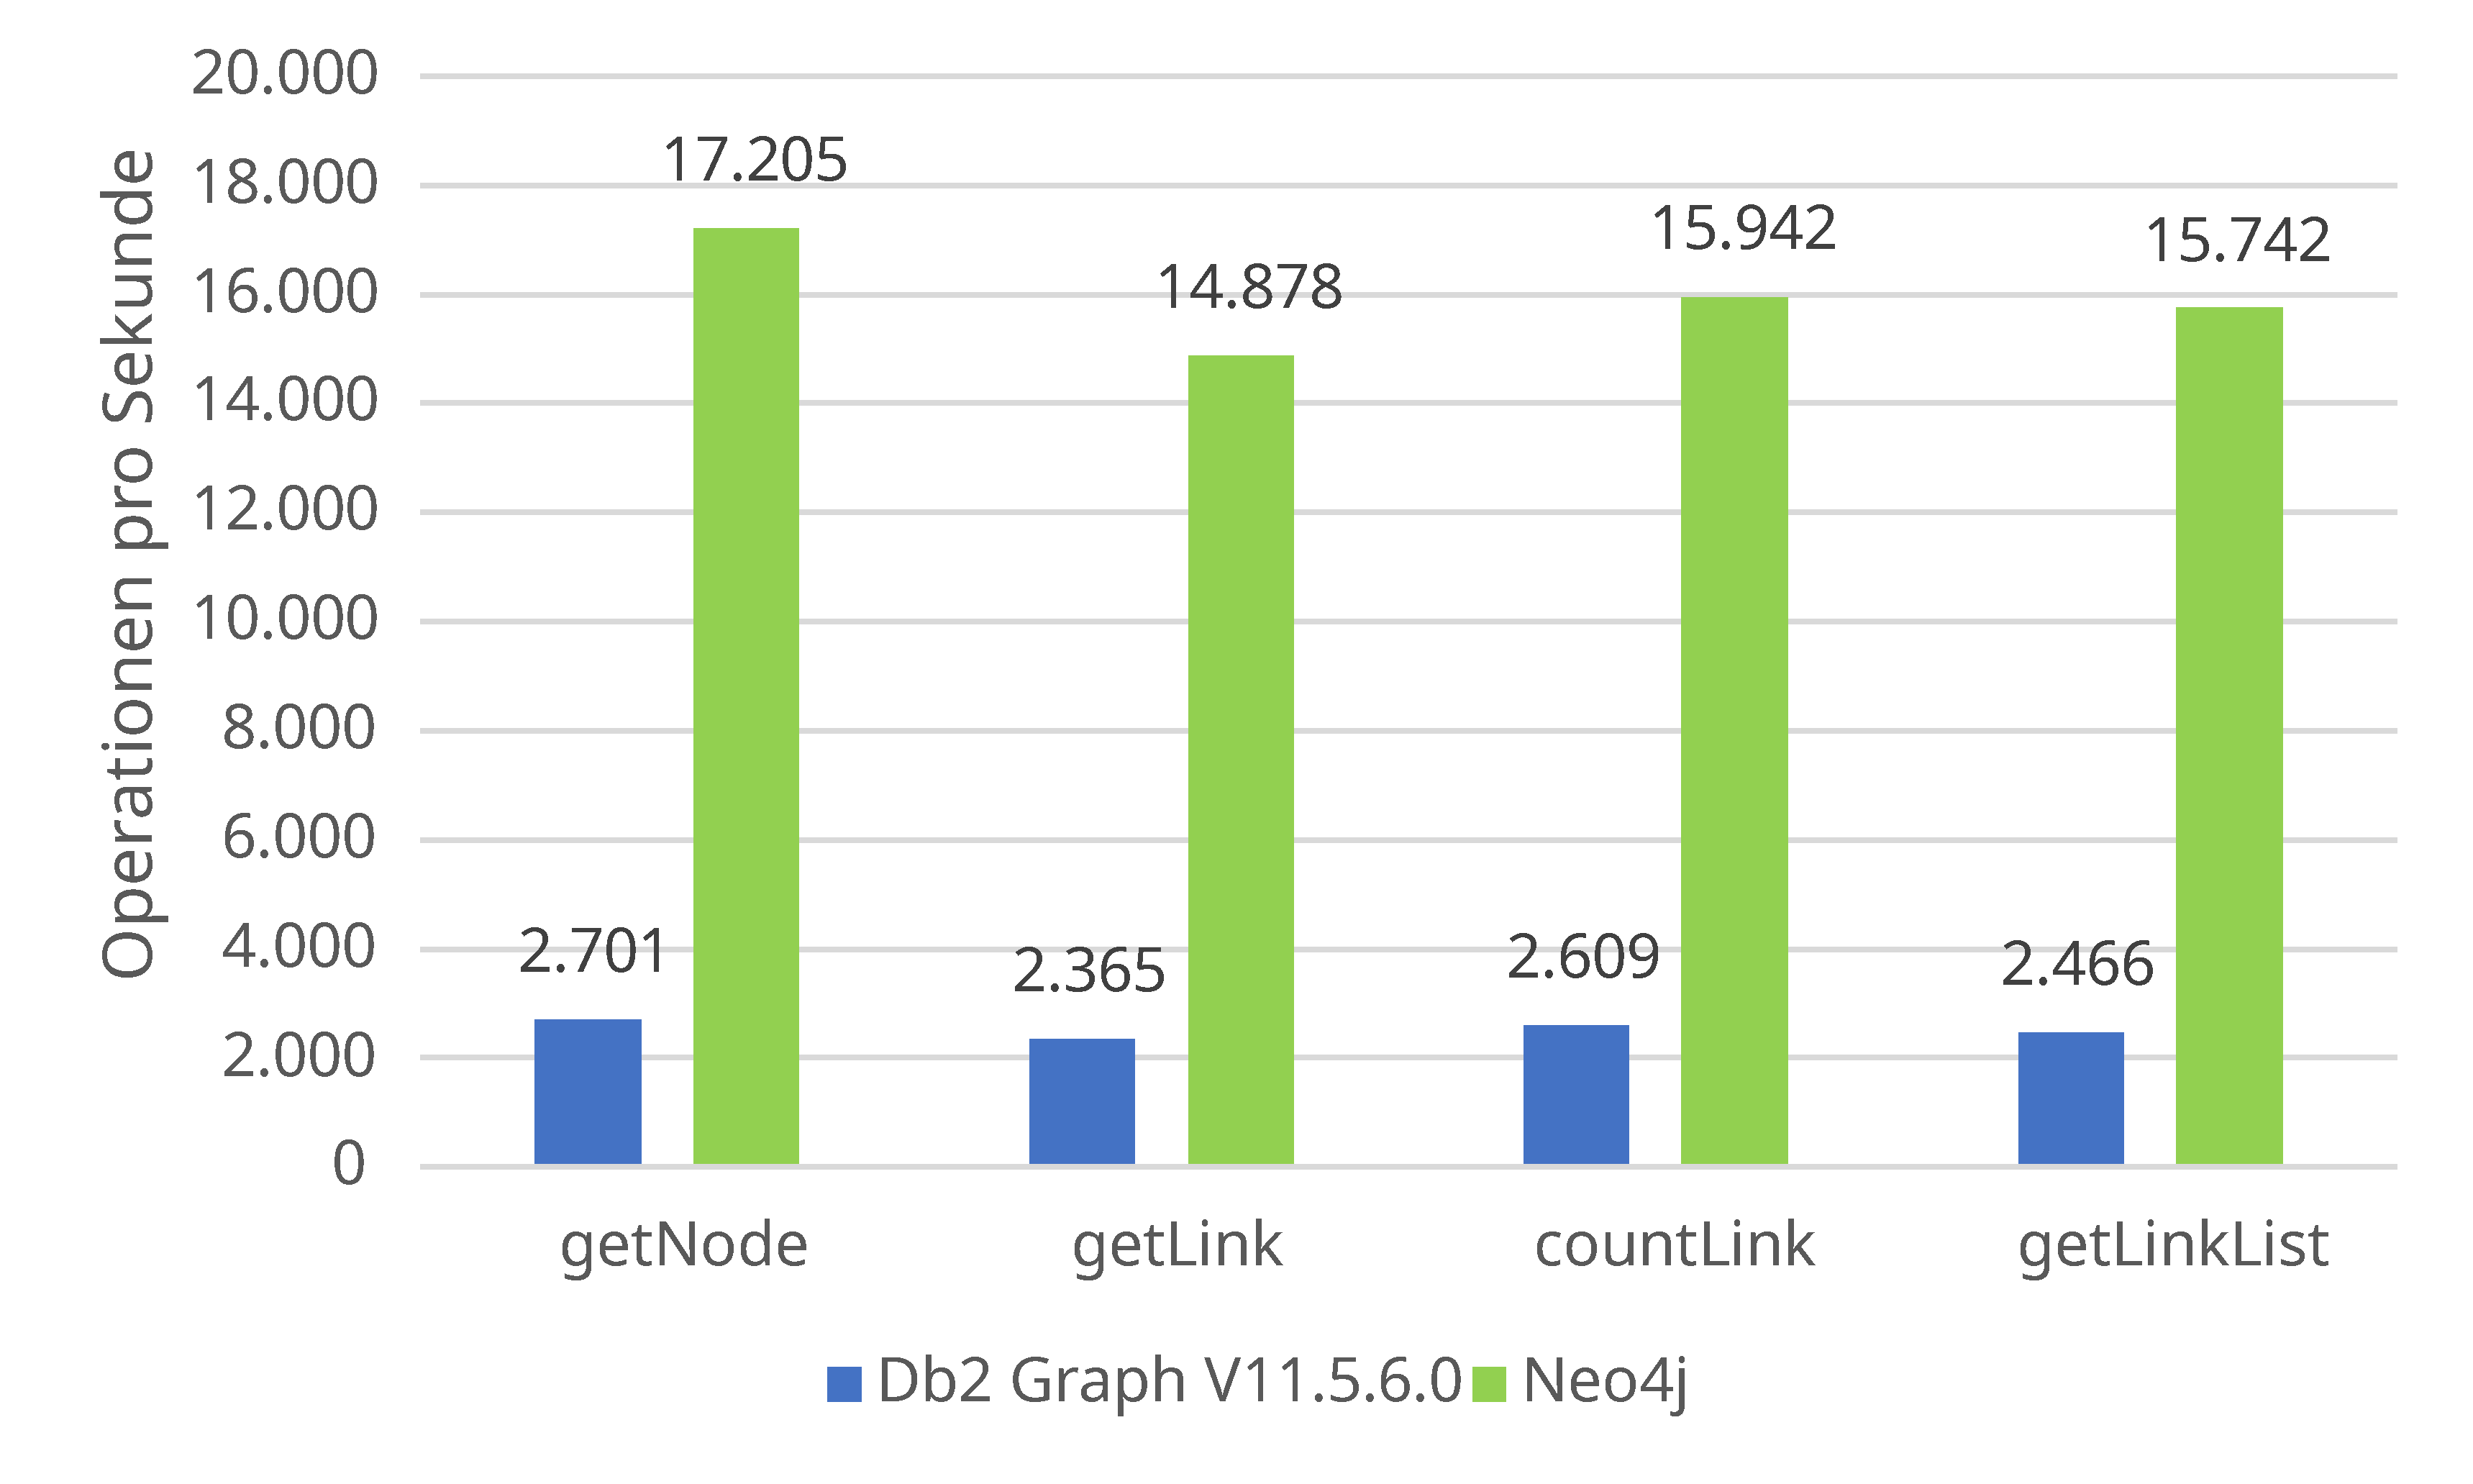
\includegraphics[width=\textwidth]{images/diagramme/linkbench_100m_real_durchsatz.pdf}
    \caption{Ergebnisse Durchsatz Linkbench-10M-Real}
    \label{fig:durchsatz:linkbench_100m_real}
    \vspace{1em}
    \textit{Die bei getLinkList abgebildeten Werte repräsentieren die Ergebnisse, die mit einer Begrenzung der Ergebnismenge auf maximal 100 Elemente erzielt werden.}
\end{figure}

\begin{figure}[!ht]
    \centering
    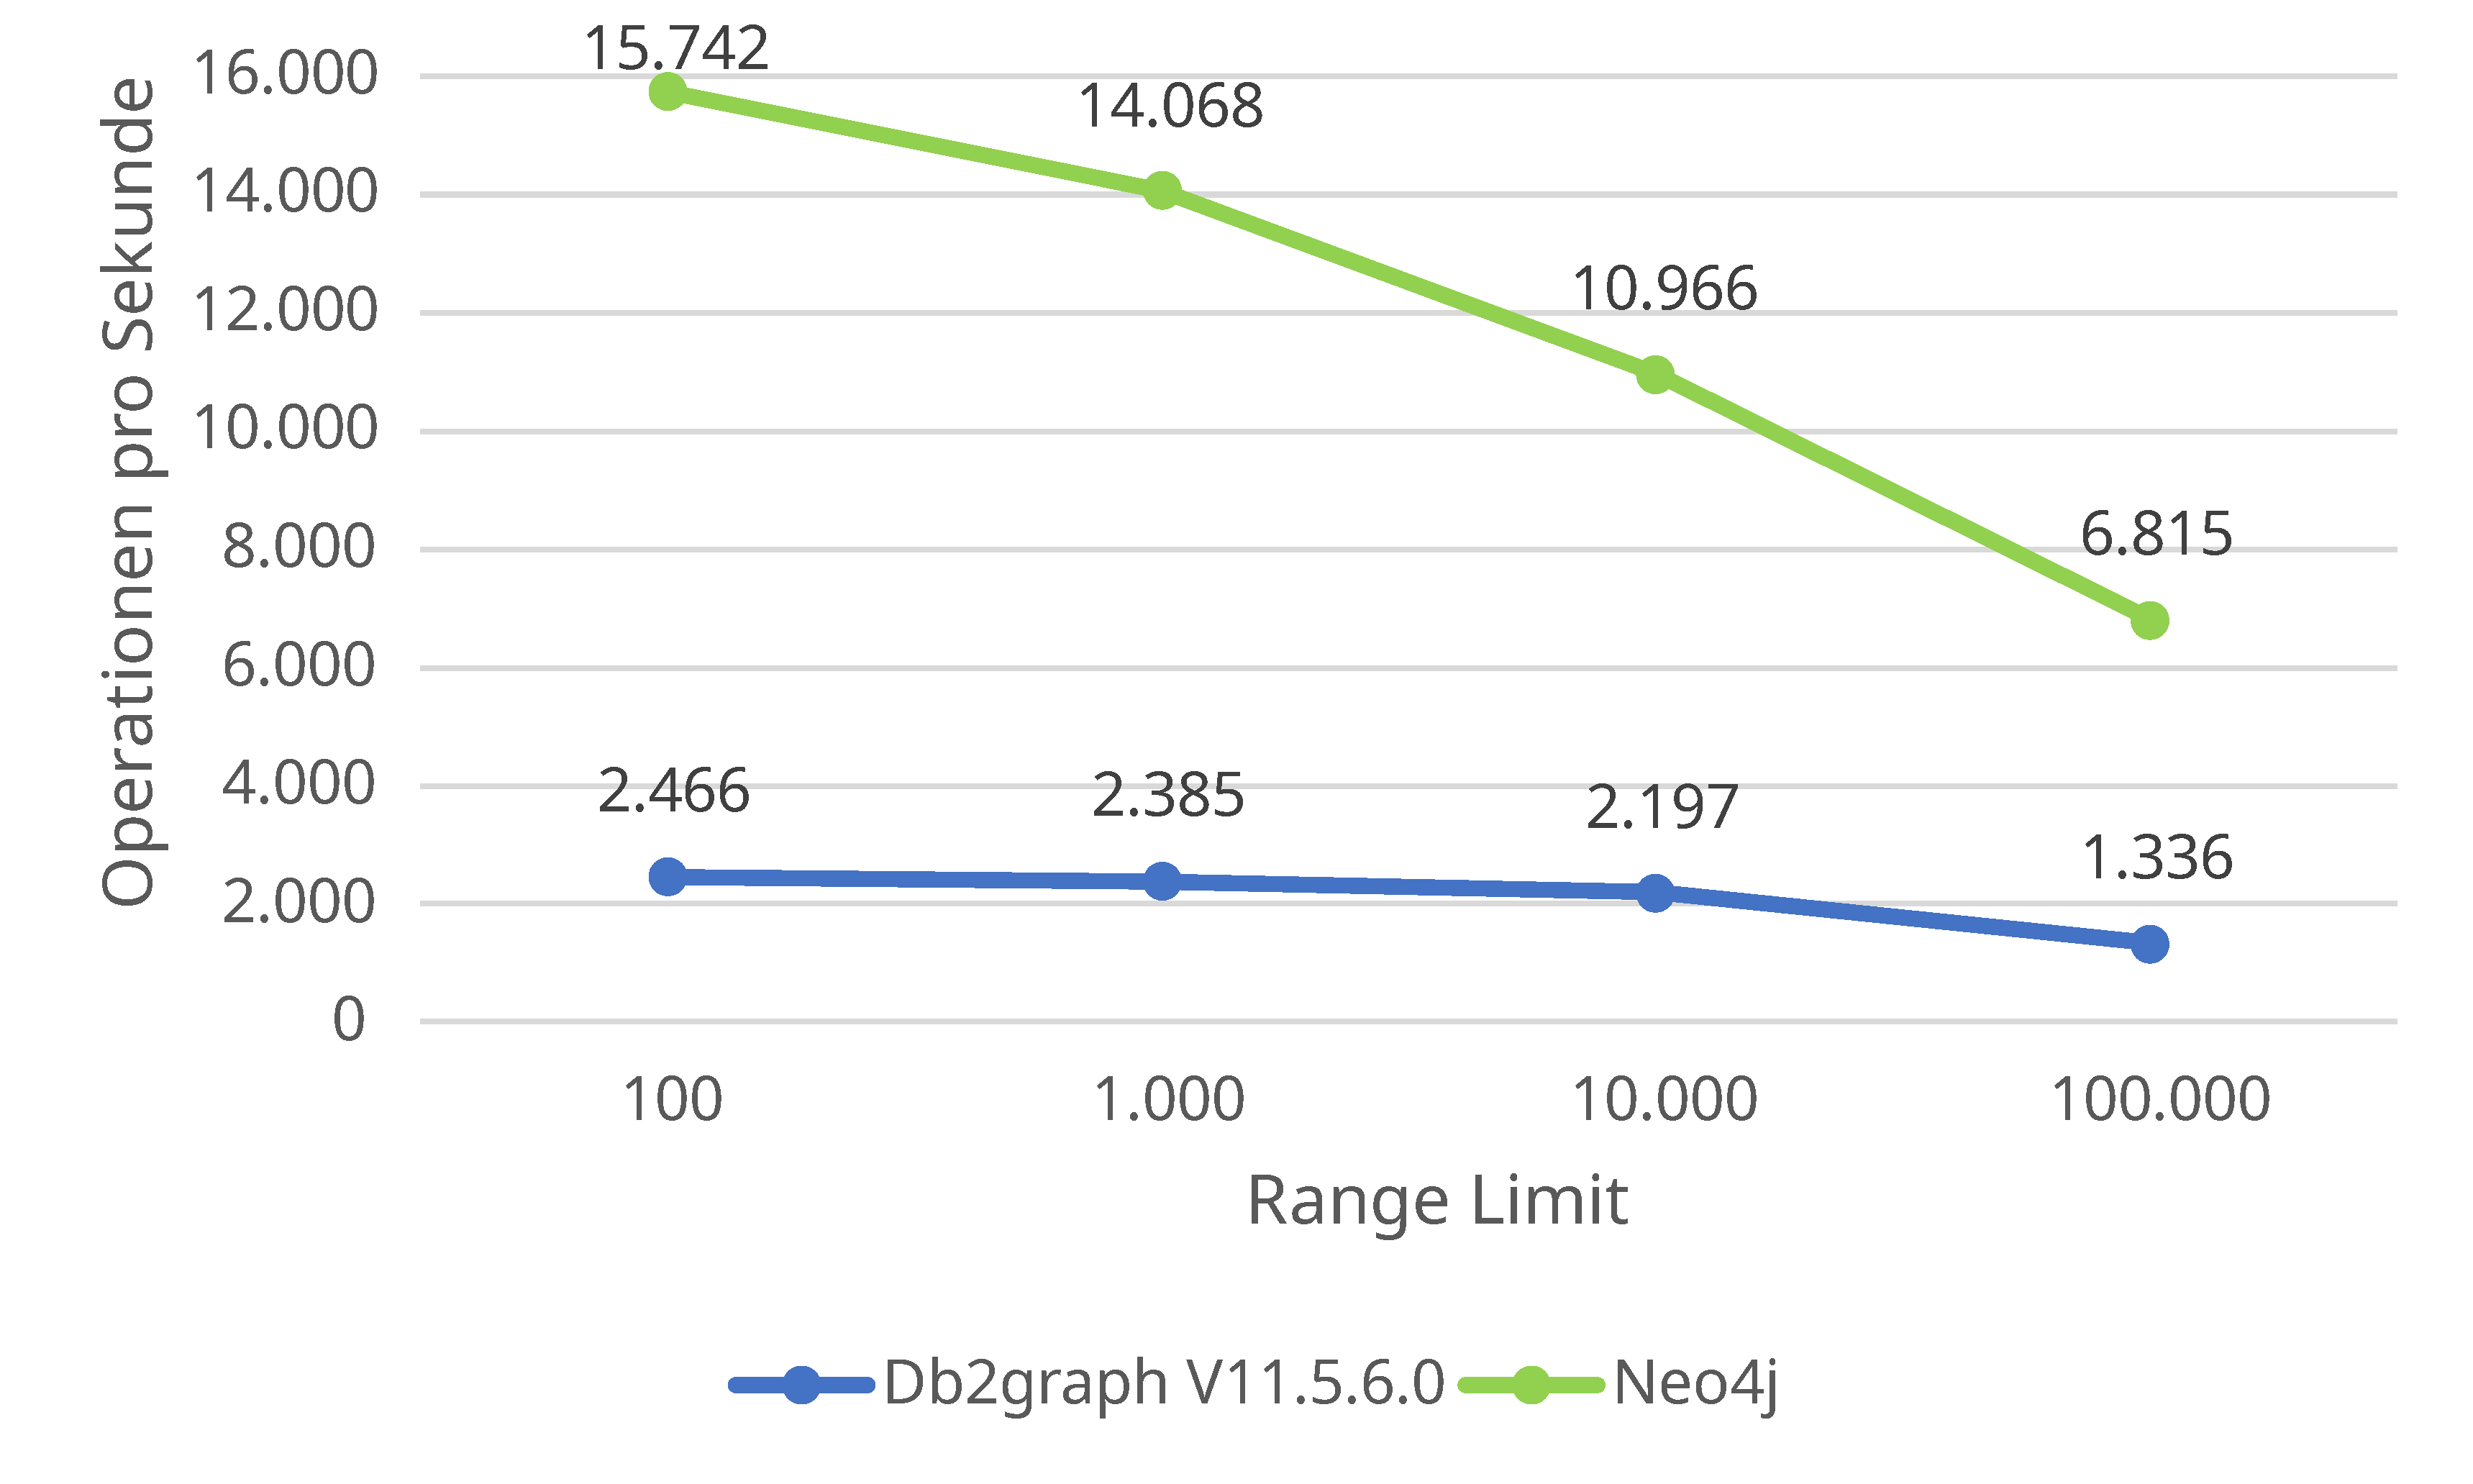
\includegraphics[width=\textwidth]{images/diagramme/limit_absolute_durchsatz_real_100m.pdf}
    \caption{Ergebnisse Durchsatz Linkbench-10M-Real getLinkList}
    \label{fig:durchsatz:linkbench_100m_real:rl}
\end{figure}